% !TEX program = xelatex
\documentclass[UTF8]{ctexart}

\RequirePackage{amsmath}
\RequirePackage{mhchem}

\RequirePackage{inputenc}
\RequirePackage{fontspec}
\RequirePackage{xeCJK}

\RequirePackage{tikz}
\RequirePackage{circuitikz}

\RequirePackage{multirow}

\RequirePackage{upgreek}

\RequirePackage{subfigure}

\RequirePackage{mathrsfs}

\setmainfont{Times New Roman}

\setCJKmainfont{等线}
\setCJKsansfont{等线}
\setCJKmonofont{等线}

\newcommand*{\dif}{\mathop{}\!\mathrm{d}}

\usepackage{geometry}
\geometry
{
    left=1.25in,
    right=1.25in,
    top=1in,
    bottom=1in
}

\title{物理笔记}
\author{李宇轩}
\date{2019.07.25}

\begin{document}
\maketitle

\newpage

\tableofcontents

\newpage

\setlength{\parindent}{0pt}

\newpage

\section{基本物理量}

\subsection{时间}
    时间符号:$t$\\[1mm]
    时间单位:s~~秒\\

\subsection{长度}
    长度符号:$s$\\[1mm]
    长度单位:m~~米\\

\subsection{质量}
    质量符号:$m$\\[1mm]
    质量单位:kg~~千克\\

\subsection{电流}
    电流符号:$I$\\[1mm]
    电流单位:A~~安培\\

\subsection{温度}
    温度符号:$T$\\[1mm]
    温度单位:K~~开尔文\\

\subsection{物质的量}
    物质的量符号:$n$\\[1mm]
    物质的量单位:mol~~摩尔

\newpage

\section{力学}

\subsection{位移}
    位移形容了物体位置的变化,是一个矢量,通常用符号$s$表示,单位是m。\\[3mm]
    位移和路程是两个不同的物理量:\\[1mm]
    路程衡量的是物体运动轨迹的长短,是一个标量。\\[1mm]
    位移衡量的是物体位置变化的多少,是一个矢量。\\[3mm]
    例如一个人绕着跑道跑了一圈,
    他的路程就是跑道的长度,但是他的位移却是零,
    因为他虽然绕操场了一圈,它的位置却并没有改变。

\subsection{速度}
    速度形容了物体位移变化的快慢,是一个矢量,通常用符号$v$表示,单位是m/s。\\[3mm]
    速度衡量了物体在一段极短的时间内位移的变化,
    所以速度等于位移对时间的导数:\\
    \begin{large}
        \begin{equation*}
            v=\frac{\dif s}{\dif t}
        \end{equation*}
    \end{large}\\
    位移是速度在时间上的累积,
    所以位移等于速度对时间的积分:\\
    \begin{large}
        \begin{equation*}
            s=\int v\cdot\dif t
        \end{equation*}
    \end{large}\\
    速度$v$的的方向始终与位移的瞬时变化量$ds$的方向相同,但与位移$s$的方向无关。

\subsection{加速度}
    加速度形容了物体速度变化的快慢,是一个矢量,通常用符号$a$表示,单位是m/s$^2$。\\[3mm]
    加速度衡量了物体在一段极短的时间内速度的变化,
    所以加速度等于速度对时间的导数:\\
    \begin{large}
        \begin{equation*}
            a=\frac{\dif v}{\dif t}
        \end{equation*}
    \end{large}\\
    速度是加速度在时间上的累积,
    所以速度等于加速度对时间的积分:\\
    \begin{large}
        \begin{equation*}
            v=\int a\cdot\dif t
        \end{equation*}
    \end{large}\\
    加速度$a$的的方向始终与速度的瞬时变化量$dv$的方向相同,但与速度$v$的方向无关。

\newpage

\subsection{匀加速直线运动}
    对于匀加速直线运动,其加速度$a$为常数。\\[3mm]
    通过对物体的加速度积分,我们可以得到物体的速度:\\
    \begin{align}
        v
        &=\int a\cdot\dif t\\[2mm]
        &=a\cdot t+v_0
    \end{align}\\
    物体的速度:
    \begin{large}
        \begin{equation*}
            v=a\cdot t+v_0
        \end{equation*}
    \end{large}\\[3mm]
    通过对物体的速度积分,我们可以得到物体的位移:\\
    \begin{align}
        s
        &=\int v\cdot\dif t\\[2mm]
        &=\int (v_0+a\cdot t)\cdot\dif t\\[1mm]
        &=v_0\cdot t+a\cdot\frac{t^2}{2}+s_0\\[3mm]
        &=\frac{a}{2}\cdot t^2+v_0\cdot t+s_0
    \end{align}\\
    物体的位移:
    \begin{large}
        \begin{equation*}
            s=\frac{a}{2}\cdot t^2+v_0\cdot t+s_0
        \end{equation*}
    \end{large}\\[5mm]
    由此我们得到了当加速度为常数时,
    求解速度和位移的方法。
    但是上述两个公式中均包含变量时间,
    而有些时候,我们并不知道时间。
    通过对以上公式的一些变换,
    我们可以得到一个只关于位移,速度,加速度的等式。

\newpage

    首先从速度公式出发:
    \setcounter{equation}{0}
    \begin{align}
        &v=v_0+a\cdot t\\[4mm]
        &v^2=\left(v_0+a\cdot t\right)^2\\[4mm]
        &v^2=v_0^2+a^2t^2+2\cdot v_0\cdot at\\[4mm]
        &v^2-v_0^2=a^2t^2+2\cdot v_0\cdot at
    \end{align}\\
    然后从位移公式出发:
    \begin{align}
        &s=\frac{a}{2}\cdot t^2+v_0\cdot t+s_0\\[4mm]
        &s-s_0=\frac{a}{2}\cdot t^2+v_0\cdot t\\[4mm]
        &2a\cdot(s-s_0)=2a\cdot\left(\frac{a}{2}\cdot t^2+v_0\cdot t\right)\\[4mm]
        &2a\cdot(s-s_0)=2a\cdot\left(\frac{a}{2}\cdot t^2\right)+2a\cdot(v_0\cdot t)\\[4mm]
        &2a\cdot(s-s_0)=a^2t^2+2\cdot v_0\cdot at
    \end{align}\\
    将两者的结果联立,得到等式:
    \begin{large}
        \begin{equation*}
            v^2-v_0^2=2a\cdot(s-s_0)
        \end{equation*}
    \end{large}

\newpage

\subsection{力}
    力衡量了物体对物体的作用大小,是一个矢量。\\[4mm]
    力符号:$F$\\[1mm]
    力单位:N~~牛顿\\[4mm]
    力单位牛顿的定义:
    N $=$ kg $\cdot$ m / s$^2$\\[2mm]
    使$1$千克的物体获得$1$~m/s$^2$的加速度
    所需的力称为$1$牛顿。\\[5mm]
    力对物体的作用效果表现为两种,一是使受力物体发生形变,二是改变受力物体的运动状态。\\[2mm]
    力的作用效果取决于三个特征,力的大小,力的方向,力的作用点。\vspace{5pt}

\subsubsection{重力}
    重力指的是物体由于地球的吸引而受到的力,通常用字母$G$表示。\\[2mm]
    重力的方向总是竖直向下,总是垂直于当地的水平面。\\[4mm]
    重力的计算公式:
    \begin{large}
        \begin{equation*}
            G=m\cdot g
        \end{equation*}
    \end{large}\\
    其中$g$为当地的重力加速度,物体所受重力的大小和质量成正比。\vspace{8pt}

\subsubsection{弹力}
    弹力指的是物体由于发生形变而产生的力,通常用字母$N$表示。\\[2mm]
    弹力的方向总是与物体发生形变的方向相反,或者说与使物体发生形变的力的方向相反。\\[4mm]
    弹力的计算公式:
    \begin{large}
        \begin{equation*}
            F=-k\cdot x
        \end{equation*}
    \end{large}\\
    其中$k$为弹簧的劲度系数,物体所受弹力的大小和形变程度成正比。\\[3mm]
    需要指出的是,在物理中弹力的覆盖面是非常广的,
    包含了弹簧由于发生显著形变产生的弹力,
    也包含了桌面由于发生微小形变产生的支持力,
    但是上述公式中的弹力仅指由弹簧产生的弹力,
    一般的弹力目前可以理解为与使物体发生形变的力大小相同。\\[3mm]
    该规律也被称为胡克定律。

\newpage

\subsubsection{摩擦力}
    摩擦力指的是两个粗糙物体由于相互摩擦而产生的力,通常用字母$f$表示。\\[2mm]
    摩擦力具体可以分为两种:滑动摩擦力和静摩擦力。\\[5mm]
    \textbf{1.动摩擦力}\\[2mm]
    滑动摩擦力指的是两个粗糙物体由于相对滑动而产生的力,通常用$f_k$表示。\\[2mm]
    滑动摩擦力的方向总是沿着接触面的切线方向,且与物体相对运动方向相反。\\[4mm]
    滑动摩擦力的计算公式:
    \begin{large}
        \begin{equation*}
            f_{k}=\mu_k\cdot N
        \end{equation*}
    \end{large}\\
    其中$\mu_k$为动摩擦系数,物体所受动摩擦力的大小和物体间的弹力成正比。\\[8mm]
    \textbf{2.静摩擦力}\\[2mm]
    静摩擦力指的是两个粗糙物体由于相对滑动趋势而产生的力,通常用$f_s$表示。\\[2mm]
    静摩擦力的方向总是沿着接触面的切线方向,且与物体的相对运动趋势方向相反。\\[2mm]
    静摩擦力的大小与物体间弹力无关,而是与外力的大小相同,使得物体始终保持静止,
    随着外力逐渐增大,物体所受的静摩擦力会逐渐增大,直至物体发生运动,
    我们将物体在发生运动前可以产生的最大的静摩擦力称为最大静摩擦力。\\[4mm]
    最大静摩擦力的计算公式:
    \begin{large}
        \begin{equation*}
            f_{sm}=\mu_{s}\cdot N
        \end{equation*}
    \end{large}\\
    其中$\mu_s$为静摩擦系数,物体所受最大静摩擦力的大小和物体间的弹力成正比。\\[4mm]
    动摩擦因数$\mu_k$和静摩擦因数$\mu_s$均是表征物体表面粗糙程度的物理量,
    实验结果表明,在同样的两个物体间,静摩擦因数通常大于动摩擦因数,即$\mu_s>\mu_k$,
    这意味者使物体开始运动所需的力通常大于维持物体匀速直线运动所需的力。

\newpage

\subsubsection{物体的平衡条件}
    我们首先需要定义力矩的概念:
    \begin{large}
        \begin{equation*}
            M=F\cdot L\cdot\sin{\theta}
        \end{equation*}
    \end{large}\\
    其中$M$代表力矩,$F$代表力,$L$代表力臂,$\alpha$代表力和力臂间的夹角。\\[3mm]
    力矩衡量了使物体转动的效果,通常用符号$M$表示,单位是N $\cdot$ m。\\[1mm]
    一般我们规定,使物体逆时针旋转的力矩为正,使物体顺时针旋转的力矩为负。\\[6mm]
    平衡是物体的一种状态,物体达到平衡状态需要满足两个条件。\\[3mm]
    \textbf{1.力的平衡}
    \begin{large}
        \begin{equation*}
            \sum{F}=0
        \end{equation*}
    \end{large}\\
    \textbf{2.力矩的平衡}
    \begin{large}
        \begin{equation*}
            \sum{M}=0
        \end{equation*}
    \end{large}\\
    需要说明的是,虽然力的三要素包含力的作用点,但是当我们在考虑力的平衡时,
    不必顾虑力的作用点不同的问题,只需要对力进行矢量叠加即可。\\[2mm]
    当物体不会发生转动时,我们只需考虑力的平衡即可(通常是对于物体所受力为共点力的情况)。\\[2mm]
    当物体不会发生平动时,我们只需考虑力矩的平衡即可(通常是对于物体有固定转动轴的情况)。\\[3mm]
    通常情况下,我们需要考虑的情况都是共点力的平衡,同时力的个数也不会超过三个,
    拉密定理形容了三个共点力情况下受力平衡的条件。\\[2mm]
    \textbf{拉密定理:}当三个共点力的合力为零时,其中任意一个力与其它两个力夹角正弦的比值相等。

\newpage

\subsection{牛顿运动定律}

\subsubsection{牛顿第一定律}
    \textbf{牛顿第一定律:}任何物体都将保持静止或匀速直线运动,
    直到外力迫使它改变这种状态为止。\\[3mm]
    牛顿第一定律说明了物体会自发的保持其运动状态,
    否定了力是维持物体运动状态的原因,
    肯定了力是改变物体运动状态的原因,
    打破了自亚里士多德以来对力的错误认识。\vspace{8pt}

\subsubsection{牛顿第二定律}
    \textbf{牛顿第二定律:}当力作用于物体时,
    物体加速度的大小,与物体所受作用力成正比,与物体的质量成反比,
    加速度的方向与所受合力的方向一致。\\[3mm]
    牛顿第二定律建立了加速度和力的关系,
    定量的说明了力对物体运动状态的改变,
    将研究力的力学和研究运动的运动学联系在了一起。\\[3mm]
    通过上述规律,我们可以发现力的大小是和加速度和质量成正比的,
    当选取合适的力的单位时,两者比例系数可以变为$1$从而被消去。\\[3mm]
    牛顿第二定律的数学表达:
    \begin{large}
        \begin{equation*}
            F=m\cdot a
        \end{equation*}
    \end{large}
    \vspace{-10pt}

\subsubsection{牛顿第三定律}
    \textbf{牛顿第三定律:}相互作用的两个物体之间的作用力和反作用力总是大小相等,方向相反。\\[3mm]
    牛顿第三定律说明了作用力和反作用力总是同时存在的,不可能单独出现的,
    一个物体在作为施力物体的同时,也必然同时作为受力物体。\\[3mm]
    牛顿第三定律的数学表达:
    \begin{large}
        \begin{equation*}
            F_{AB}=F_{BA}
        \end{equation*}
    \end{large}

\newpage

\subsubsection{惯性系和非惯性系}
    考虑这样一个场景,在一个封闭的车厢中有一个人和一个小球,
    当汽车突然向右加速时,车厢中的人观察到小球向左加速。
    然而小球却没有受到水平方向的力,为何会有加速度呢?
    这是由于参照系的选取造成的,小球相对于地面实际上并没有加速度,
    观察者得出小球有加速度的结论是由于其将车厢作为参照系造成的。\\[6mm]
    从这个例子中,我们可以抽象出惯性系何非惯性系的概念。\\[2mm]
    惯性系:以加速度为零的物体作为参照物的参照系。\\[2mm]
    非惯性系:以加速度不为零的物体作为参照物的参照系。\\[2mm]
    根据观察者的结论,我们发现牛顿运动定律,只适用于惯性系,不适用于非惯性系。\\[6mm]
    为了解决实际问题,我们可以在非惯性系中添加一个虚拟的力,
    以补偿非惯性系带来的效应,使其等效为一个惯性系,从而可以应用牛顿运动定律。\\[3mm]
    我们做出如下规定:在任何具有加速度$a$的参照系中研究问题时,对每一个质量为$m$的物体施加一个力,
    力的大小是$ma$,力的方向与$a$相反,这个力被称为非惯性力。\\[3mm]
    需要注意的是,非惯性力是一个假象的力,即没有施力物体,也没有反作用力。\\[7mm]
    通过非惯性力的思想,我们可以简单的解释超重和失重的现象。\\[3mm]
    在过山车加速上升的过程中,人获得了一个竖直向上的加速度,
    此时人受到了竖直向下的非惯性力和竖直向下的重力,两者叠加,
    人会感觉到自己变得更重,这就是超重的现象。\\[3mm]
    在过山车加速下降的过程中,人获得了一个竖直向下的加速度,
    此时人受到了竖直向上的非惯性力和竖直向下的重力,两者叠加,
    人会感觉到自己变得更轻,这就是失重的现象。

\newpage

\subsection{功}
    功衡量了做功的多少,是一个标量。\\[4mm]
    功符号:$W$\\[1mm]
    功单位:J~~焦耳\\[4mm]
    功单位焦耳的定义:
    J $=$ N $\cdot$ m\qquad J $=$ kg $\cdot$ m/s$^2\cdot$ m\\[2mm]
    使$1$千克的物体保持$1$~m/s$^2$的加速度移动$1$米所做的功称为$1$焦耳。\\[4mm]
    功是力在空间上的积累,所以功等于力对位移的积分:\\[3mm]
    功的计算公式(变力做功):
    \begin{large}
        \begin{equation*}
            W=\int_{s_1}^{s_2} F\cdot \dif s
        \end{equation*}
    \end{large}\\
    功的计算公式(恒力做功):
    \begin{large}
        \begin{equation*}
            W=F\cdot s
        \end{equation*}
    \end{large}
    \vspace{-20pt}
    
\subsection{功率}
    功率衡量了做功的快慢,是一个标量。\\[4mm]
    功率符号:$P$\\[1mm]
    功率单位:W~~瓦特\\[4mm]
    功率单位瓦特的定义:
    W $=$ J/s\qquad W $=$ N $\cdot$ m/s\\[2mm]
    在$1$秒内做功$1$焦耳称为$1$瓦特。\\[4mm]
    功率是单位时间内所做的功,所以功率等于功对时间导数:\vspace{15pt}
    \setcounter{equation}{0}
    \begin{align}
        P
        =\frac{\dif W}{\dif t}
        &=\frac{\dif}{\dif t}\cdot\int F\cdot s\\[3mm]
        &=\frac{\dif}{\dif t}\cdot\int F\cdot v\cdot \dif t\\[3mm]
        &=F\cdot v
    \end{align}\\
    功率的计算公式:
    \begin{large}
        \begin{equation*}
            P=F\cdot v
        \end{equation*}
    \end{large}

\newpage

\subsection{能量}
    能量衡量了物体做功本领的强弱。\\[4mm]
    能量符号:$E$\\[1mm]
    能量单位:J~~焦耳\\[4mm]
    能量单位焦耳的定义:
    J = N $\cdot$ m\qquad J = kg$\cdot$ m/s$^2$ $\cdot$ m\\[2mm]
    使$1$千克的物体保持1~m/s$^2$的加速度移动$1$米所做的功称为1焦耳。

\subsubsection{动能}
    动能指的是物体由于运动而具有的能量,通常用字母$E_k$表示。\\[3mm]
    我们由变力做功的计算公式进行推导:\vspace{5pt}
    \setcounter{equation}{0}
    \begin{align}
        W
        &=\int_L F\cdot \dif s\\[5mm]
        &=\int_L F\cdot v\cdot \dif t\\[5mm]
        &=\int_L m\cdot a\cdot v\cdot \dif t\\[5mm]
        &=\int_L m\cdot \frac{dv}{dt}\cdot v\cdot \dif t\\[5mm]
        &=\int_{v_1}^{v_2}m\cdot v\cdot \dif v\\[5mm]
        &=\frac{1}{2}\cdot m\cdot v_2\,^2-\frac{1}{2}\cdot m\cdot v_1\,^2
    \end{align}\\
    我们将物体从速度为$0$至速度为$v$间外力所做的功,定义为动能。\\[3mm]
    根据动能的定义,令$v_1=0$,令$v_2=v$,代入可得动能的计算公式。\\[5mm]
    动能的计算公式:
    \begin{large}
        \begin{equation*}
            E_k=\frac{1}{2}\cdot m\cdot v^2
        \end{equation*}
    \end{large}

\newpage

    如果我们分别用$E_{k_1}$和$E_{k_2}$表示速度为$v_1$和$v_2$时的动能:\vspace{5pt}
    \begin{align}
        W
        &=\frac{1}{2}\cdot m\cdot v_2\,^2-\frac{1}{2}\cdot m\cdot v_1\,^2\\[3mm]
        &=E_{k_2}-E_{k_1}\\[3mm]
        &=\Delta E_k
    \end{align}\\
    外力所做的功等于动能的增量(动能定理):
    \begin{large}
        \begin{equation*}
            W=E_{k_2}-E_{k_1}=\Delta E_k
        \end{equation*}
    \end{large}

\subsubsection{保守力和耗散力}
    根据力的做功特点,我们可以将力分为保守力和耗散力:\\[3mm]
    保守力:力所做的功和物体的运动路径无关。\\[2mm]
    耗散力:力所做的功和物体的运动路径有关。\\[4mm]
    重力就是一种典型的保守力,
    将一个物体从一楼运送到五楼,
    无论是坐电梯还是走楼梯,
    重力所做的功都是相同的,
    所以重力就是一种保守力。\\[3mm]
    摩擦力是一种典型的耗散力,
    由于摩擦力的方向始终和运动方向相同,
    将一个物体在一个粗糙的平面上从一个位置移动到另一个位置,
    当物体的运动路径分别是直线和曲线时,
    显然摩擦力所做的功与物体移动的路径长度有关,
    所以摩擦力是一种耗散力。\\

\subsubsection{重力势能}
    重力势能是指的是物体由于重力而具有的能量,通常用字母$E_p$表示。\\[2mm]
    重力是一种保守力,因此受到重力的物体具有重力势能。\\[4mm]
    我们由恒力做功的计算公式进行推导:
    \setcounter{equation}{0}
    \begin{align}
        W
        &=G\cdot h\\[3mm]
        &=m\cdot g\cdot (h_1-h_2)\\[3mm]
        &=m\cdot g\cdot h_1-m\cdot g\cdot h_2
    \end{align}

\newpage

    我们将物体从高度为$h$处至高度为$0$处重力所做的功,定义为重力势能。\\[3mm]
    根据重力势能的定义,令$h_1=h$,令$h_2=0$,代入可得重力势能的计算公式。\\[5mm]
    重力势能的计算公式:
    \begin{large}
        \begin{equation*}
            E_p=m\cdot g\cdot h
        \end{equation*}
    \end{large}\\
    如果我们分别用$E_{p_1}$和$E_{p_2}$表示高度为$h_1$和$h_2$时的重力势能:\vspace{5pt}
    \begin{align}
        W
        &=m\cdot g\cdot h_1-m\cdot g\cdot h_2\\[3mm]
        &=-(E_{p_2}-E_{p_1})\\[3mm]
        &=-\Delta E_p
    \end{align}\\
    重力所做的功等于重力势能的负增量:
    \begin{large}
        \begin{equation*}
            W=-(E_{p_2}-E_{p_1})=-\Delta E_p
        \end{equation*}
    \end{large}

\subsubsection{弹性势能}
    弹性势能是指的是物体由于弹性力而具有的能量,通常用字母$E_p$表示。\\[2mm]
    弹性力是一种保守力,因此受到弹性力的物体具有弹性势能。\\[4mm]
    我们由变力做功的计算公式进行推导:\vspace{5pt}
    \setcounter{equation}{0}
    \begin{align}
        W
        &=\int_{x_1}^{x_2} F\cdot dx\\[3mm]
        &=\int_{x_1}^{x_2} -k\cdot x\cdot dx\\[3mm]
        &=-\int_{x_1}^{x_2} k\cdot x\cdot dx\\[3mm]
        &=-\left(\frac{1}{2}\cdot k\cdot x_2\,^2-\frac{1}{2}\cdot k\cdot x_1\,^2\right)\\[3mm]
        &=\frac{1}{2}\cdot k\cdot x_1\,^2-\frac{1}{2}\cdot k\cdot x_2\,^2
    \end{align}

\newpage

    我们将物体从位移为$x$处至位移为$0$处弹性力所做的功,定义为弹性势能。\\[3mm]
    根据弹性势能的定义,令$x_1=x$,令$x_2=0$,代入可得弹性势能的计算公式。\\[5mm]
    弹性势能的计算公式:
    \begin{large}
        \begin{equation*}
            E_p=\frac{1}{2}\cdot k\cdot x^2
        \end{equation*}
    \end{large}\\
    如果我们分别用$E_{p_1}$和$E_{p_2}$表示位移为$x_1$和$x_2$时的弹性势能:\vspace{5pt}
    \begin{align}
        W
        &=\frac{1}{2}\cdot k\cdot x_1\,^2-\frac{1}{2}\cdot k\cdot x_2\,^2\\[3mm]
        &=-(E_{p_2}-E_{p_1})\\[3mm]
        &=-\Delta E_p
    \end{align}\\
    弹性力所做的功等于弹性势能的负增量:
    \begin{large}
        \begin{equation*}
            W=-(E_{p_2}-E_{p_1})=-\Delta E_p
        \end{equation*}
    \end{large}

\subsubsection{机械能和机械能守恒定律}
    机械能是物体动能和势能的总和。\\[3mm]
    \textbf{机械能守恒定律:}
    在只有保守力做功的情况下,
    势能和动能可以相互转化,
    但机械能不变。\\[3mm]
    机械能守恒定律的数学表达:
    \begin{large}
        \begin{equation*}
            E_{k_1}+E_{p_1}=E_{k_2}+E_{p_2}
        \end{equation*}
    \end{large}\\
    通过机械能守恒定律,我们还能更好的理解保守力和耗散力:\\[4mm]
    1.保守力做功,机械能不变。\\[2mm]
    例如在自由落体运动中,重力做功,
    物体的重力势能转化为了物体的动能,
    机械能没有变化。\\[3mm]
    例如在单摆运动中,重力做功,
    物体的重力势能和物体的动能间相互转化,
    机械能没有变化。\\[4mm]
    2.耗散力做功,机械能减少。\\[2mm]
    例如有一定速度的物体在一个粗糙平面上滑动,
    摩擦力做功,物体的势能不变,物体的动能减小,
    机械能被消耗,以热量的形式放出。

\newpage

\subsection{动量}
    冲量衡量了力在时间上的积累效果,是一个矢量,通常用符号$I$表示,单位是N$\cdot$s。\\[3mm]
    冲量是力在时间上的积累,所以冲量等于力对时间的积分:\\[3mm]
    冲量的计算公式(变力的冲量):
    \begin{large}
        \begin{equation*}
            I=\int_{t_1}^{t_2}F\cdot\dif t
        \end{equation*}
    \end{large}\\
    冲量的计算公式(恒力的冲量):
    \begin{large}
        \begin{equation*}
            I=F\cdot t
        \end{equation*}
    \end{large}\\
    动量衡量了物体运动的强弱,是一个矢量,通常用符号$P$表示,单位是kg$\cdot$m/s。\\[3mm]
    动量的计算公式:
    \begin{large}
        \begin{equation*}
            P=m\cdot v
        \end{equation*}
    \end{large}
    \vspace{-10pt}
    
\subsubsection{动量定理}
    我们由牛顿第二定律进行推导:
    \setcounter{equation}{0}
    \begin{align}
        F
        &=m\cdot a\\[4mm]
        &=m\cdot\frac{\dif v}{\dif t}\\[4mm]
        &=\frac{\dif(m\cdot v)}{\dif t}\\[4mm]
        &=\frac{\dif P}{\dif t}
    \end{align}\\
    将该结论代入冲量的计算公式可得:
    \begin{align}
        I
        &=\int_{t_1}^{t_2}~F\cdot\dif t\\[4mm]
        &=\int_{P_1}^{P_2}~\frac{\dif P}{\dif t}\cdot\dif t\\[4mm]
        &=\int_{P_1}^{P_2}~\dif P\\[4mm]
        &=P_2-P_1
    \end{align}

\newpage

    \textbf{动量定理:}物体所受合外力的冲量等于动量的增量。\\[3mm]
    动量定理的数学表达:
    \begin{large}
        \begin{equation*}
            I=P_2-P_2=\Delta t
        \end{equation*}
    \end{large}\\
    上述推导中第四步得出的结论,
    实际上是牛顿第二定律的另一表达形式,
    即力是动量关于时间的导数,
    该形式也是牛顿最初提出牛顿第二定律时的表述。\\[3mm]
    力是动量关于时间的导数:
    \begin{large}
        \begin{equation*}
            F=\frac{\dif P}{\dif t}
        \end{equation*}
    \end{large}
    \vspace{-10pt}

\subsubsection{动量守恒定律}
    设一个体系内有两个物体,且该体系不受外力:\\[3mm]
    1.物体的质量分别为$m_a$和$m_b$\\[2mm]
    2.在$t_1$时刻两个物体的速度分别为$v_{a_1}$和$v_{b_1}$\\[2mm]
    3.在$t_2$时刻两个物体的速度分别为$v_{a_2}$和$v_{b_2}$\\[2mm]
    4.物体$m_a$和物体$m_b$分别受到来自对方的内力$F_{ba}$和$F_{ab}$\\[4mm]
    根据动量定理可以得到:
    \setcounter{equation}{0}
    \begin{align}
        &\int_{t_1}^{t_2}F_{ba}\cdot \dif t=m_a\cdot v_{a_2}-m_a\cdot v_{a_1}=\Delta I_a\\[4mm]
        &\int_{t_1}^{t_2}F_{ab}\cdot \dif t=m_b\cdot v_{b_2}-m_b\cdot v_{b_2}=\Delta I_b
    \end{align}\\
    两式相加可得:
    \begin{align}
        &\int_{t_1}^{t_2}\left(F_{ba}+F_{ab}\right)\cdot\dif t=\Delta I_a+\Delta I_b\\[4mm]
        &\int_{t_1}^{t_2}\left(F_{ba}+F_{ab}\right)\cdot\dif t=\Delta I
    \end{align}\\
    我们由牛顿第三定律可知:
    \begin{align}
        &F_{ba}+F_{ab}=0\\[3mm]
        &\Delta I=0
    \end{align}\\
    \textbf{动量守恒定律:}当体系受到的合外力为零时,则系统的总动量不变。

\newpage

\subsection{匀速圆周运动}
    对于匀速圆周运动,其线速度$v$为常数。\\[4mm]
    我们会通过以下四个物理量来描述一个匀速圆周运动:\\[3mm]
    1.线速度$v$描述了物体单位时间内划过的弧长。\\[2mm]
    2.角速度$\omega$描述了物体单位时间内划过的弧度。\\[2mm]
    3.周期$T$描述了物体绕圆一周,即转动$2\pi$所需的时间。\\[2mm]
    4.转速$n$描述了物体一秒内绕圆一周的次数。\\[5mm]
    根据弧长公式$l=\alpha\cdot r$,我们可以发现角速度和线速度间仅相差一个半径:
    \begin{large}
        \begin{equation*}
            v=\omega\cdot r
        \end{equation*}
    \end{large}\\
    根据线速度的定义,线速度等于圆的周长除以周期:\\
    \begin{large}
        \begin{equation*}
            v=\frac{2\pi r}{T}
        \end{equation*}
    \end{large}\\
    根据角速度的定义,角速度等于圆的周角除以周期:\\
    \begin{large}
        \begin{equation*}
            \omega=\frac{2\pi}{T}
        \end{equation*}
    \end{large}\\
    显然,转速可以表示为周期的倒数:\\
    \begin{large}
        \begin{equation*}
            n=\frac{1}{T}
        \end{equation*}
    \end{large}\\[1mm]
    匀速圆周运动中,虽然速度大小是恒定的,
    但是速度方向是变化的,所以物体必然有加速度。\\[3mm]
    接下来将通过证明,求得匀速圆周运动中加速度的大小和方向。

\newpage

    由于速度三角形和位移三角形相似:
    \setcounter{equation}{0}
    \begin{align}
        &\frac{\dif v}{v}=\frac{\dif r}{r}
    \end{align}\\
    此处的$r$指圆周运动的半径,此处的$v$指圆周运动的线速度($v=v_a=v_b$)。\\[3mm]
    等式两边同时除以$\dif t$可得:
    \begin{align}
        &\frac{\dif v}{v\cdot\dif t}=\frac{\dif r}{r\cdot\dif t}\\[4mm]
        &\frac{\dif v}{\dif t}=\frac{v}{r}\cdot\frac{\dif r}{\dif t}
    \end{align}\\
    根据加速度的定义:
    \begin{align}
        a
        &=\frac{\dif v}{\dif t}\\[4mm]
        &=\frac{v}{r}\cdot\frac{\dif r}{\dif t}\\[4mm]
        &=\frac{v^2}{r}
    \end{align}\\
    加速度的方向与速度的瞬时变化量$\dif v$相同,
    因此加速度的方向始终指向圆心。\vspace{5pt}
    \begin{figure}[h]
        \begin{center}
            \subfigure[位移三角形]
            {
                \begin{minipage}[t]{0.4\linewidth}
                    \begin{tikzpicture}[>=stealth,scale=1.5]
                        \draw(0,0) circle (2);
                        \draw(0,0)--(2,0);
                        \draw(0,0)--(1.732,1);
                        \draw [->,>=stealth](2,0)--(2,2) node at(2.3,2) {$v_a$};
                        \draw [->,>=stealth](1.732,1)--(0.60,2.804) node at(0.45,3.00) {$v_b$};
                        \draw [dashed](2,0)--(1.732,1);
                        \node at(0.6,0.15) {$\dif\theta$};
                        \node at(1.6,0.45) {$\dif r$};
                    \end{tikzpicture}
                \end{minipage}
            }\qquad\qquad\qquad\qquad
            \subfigure[速度三角形]
            {
                \begin{minipage}[t]{0.25\linewidth}
                    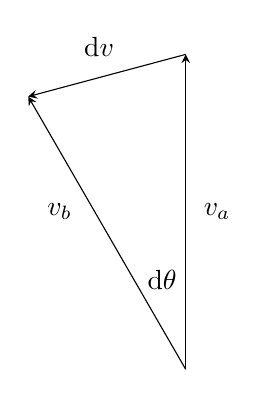
\begin{tikzpicture}[>=stealth,scale=2]
                        \draw [->,>=stealth](6,0)--(6,2) node at(6.2,1) {$v_a$};
                        \draw [->,>=stealth](6,0)--(5,1.732) node at(5.2,1) {$v_b$};
                        \draw [->,>=stealth](6,2)--(5,1.732) node at(5.45,2.05) {$\dif v$};
                        \node at(5.85,0.57) {$\dif\theta$};
                    \end{tikzpicture}
                \end{minipage}
            }
            \caption{匀速圆周运动}
        \end{center}
    \end{figure}

\newpage

    从上面的推导中我们发现,匀速圆周运动的加速度的大小为定值,加速度的方向始终指向圆心。\\[4mm]
    代入相关公式,可以得到不同形式的匀速圆周运动加速度的计算公式:\\[3mm]
    关于线速度:
    \begin{large}
        \begin{equation*}
            a=\frac{v^2}{r}
        \end{equation*}
    \end{large}\\
    关于角速度:
    \begin{large}
        \begin{equation*}
            a=\omega^2\cdot r
        \end{equation*}
    \end{large}\\
    关于周期:
    \begin{large}
        \begin{equation*}
            a=\frac{4\pi^2}{T^2}\cdot r
        \end{equation*}
    \end{large}\\
    匀速圆周运动中的加速度始终指向圆心,因此也称为向心加速度,而对应的力则称为向心力。\\[8mm]
    根据牛顿第二定律,向心力的方向始终指向圆心,向心力的大小也可以代入求得。\\[3mm]
    向心力的计算公式:
    \begin{large}
        \begin{align*}
            &F=m\cdot \frac{v^2}{r}\\[5mm]
            &F=m\cdot\omega^2\cdot r\\[5mm]
            &F=m\cdot\frac{4\pi^2}{T^2}\cdot r
        \end{align*}
    \end{large}\\
    如果在匀速圆周运动中,向心力小于应有值,物体的运动轨迹将会偏向圆心。\\[3mm]
    如果在匀速圆周运动中,向心力大于应有值,物体的运动轨迹将会偏离圆心。
    
\newpage

\section{万有引力}

\subsection{开普勒定律}

\subsubsection{开普勒第一定律}
    \textbf{开普勒第一定律:}所有行星绕太阳的轨道均是椭圆,太阳处于椭圆的一个焦点上。\\[3mm]
    开普勒在研究火星的运动轨迹的过程中发现,如果按照哥白尼的体系将火星的运动设想为匀速圆周运动,
    理论计算得到的数据与第谷观测得到的数据相差$8$分,由此发现了开普勒第一定律。\\[3mm]
    如果考虑彗星的影响,周期彗星的轨道是椭圆,非周期彗星的轨道是双曲线或抛物线,
    但这些轨道实际上均可以使用圆锥曲线统一,同时太阳始终处于圆锥曲线的焦点处。\\[3mm]
    开普勒第一定律也被称为椭圆定律。\\

\subsubsection{开普勒第二定律}
    \textbf{开普勒第二定律:}在任何相等的时间内,行星和太阳的连线扫过的面积是相等的。\\[3mm]
    开普勒在进一步研究火星的运动状态时发现,火星处于轨道上不同位置时,其运行速度不一样,远离太阳时运动的较慢,接近太阳时运动的较快,
    从中探索出了开普勒第二定律。\\[3mm]
    开普勒第二定律也被称为面积定律。\\

\subsubsection{开普勒第三定律}
    \textbf{开普勒第三定律:}绕太阳运行的各行星,轨道半长轴的立方和公转周期的平方成正比。\\[3mm]
    开普勒第三定律的数学表达:
    \begin{large}
        \begin{equation*}
            k=\frac{R^3}{T^2}
        \end{equation*}
    \end{large}\\
    其中,$R$是行星轨道的半长轴,$T$是行星的公转周期,$k$是开普勒恒量。\\[4mm]
    开普勒在研究完火星的运动规律后,不满足于此,希望寻找行星运动的共通规律,
    利用第谷对众多星体的观测数据,用了十年时间,最终揭示了开普勒第三定律。\\[3mm]
    开普勒第三定律也被称为调和定律。

\newpage

\subsection{引力}
    引力是由于质量而产生的力。\\[3mm]
    引力公式:
    \begin{large}
        \begin{equation*}
            F = G \cdot \frac{m_{1} \cdot m_{2}}{{r}^{2}} 
        \end{equation*}
    \end{large}\\
    其中$G$为引力常数:
    \begin{large}
        \begin{equation*}
            G = 6.674 \times {10}^{-11}~\text{N}\cdot\text{m}^2\text{ / kg}^2
        \end{equation*}
    \end{large}\\[2mm]
    其中我们认为:\\[3mm]
    下标为1的代表质量较大的物体。\\[2mm]
    下标为2的代表质量较小的物体。\\[3mm]
    例如研究宇宙飞船绕地球运动,
    我们应当用$m_1$代表地球质量,
    而用$m_2$代表宇宙飞船的质量。

\subsection{引力场强}
    引力场强代表了单位质量的物体在引力场中特定位置所受到的引力。\\[3mm]
    引力场强定义式:\vspace{3pt}
    \begin{large}
        \begin{equation*}
            E=\frac{F}{m_2}
        \end{equation*}
    \end{large}\\
    引力场强公式:\vspace{3pt}
    \begin{large}
        \begin{equation*}
            E=\frac{G\cdot m_{1}}{{r}^{2}}       
        \end{equation*}
    \end{large}\\
    引力场强单位:N / kg

\subsubsection{引力场强和重力加速度}
    我们使用地球的质量$m_1=5.97\times 10^{24}~\text{kg}$和半径$r=6.37\times 10^6~\text{m}$数据作为参数:\vspace{5pt}
    \setcounter{equation}{0}
    \begin{align}
        E&=6.67\times 10^{-11}\times\frac{5.97\times 10^{24}}{~\left(6.37\times 10^{6}\right)^2~}=9.8~\text{N/kg}
    \end{align}\\
    由此可见,重力加速度的本质是引力场强在地球附近的近似。\\[3mm]
    同时我们可以发现,引力场强的单位N/kg和重力加速度的单位m/s$^2$是完全等价的。

\newpage
        
\subsection{引力势能}
    引力势能是由于引力而产生的能量。\\[3mm]
    引力势能在数值上等于将物体移动到距离引力中心无穷远处引力所做的功,
    因此我们可以对引力进行积分求出引力所做的功,从而推导出引力势能的公式。\\[5mm]
    首先求解引力的反常积分:
    \setcounter{equation}{0}
    \begin{align}    
        W&=\int_{r}^{\infty} F\cdot\dif s\\[3mm]
        &= \int_{r}^{\infty} G \cdot \frac{m_{1} \cdot m_{2}}{{s}^{2}}\cdot\dif s \\[3mm]
        &=(G \cdot m_{1} \cdot m_{2}) \cdot \int_{r}^{\infty} \frac{1}{{s}^{2}}\cdot\dif s \\[3mm]
        &=(G \cdot m_{1} \cdot m_{2}) \cdot \int_{r}^{\infty} {s}^{-2}\cdot\dif s \\[3mm]
        &=(G \cdot m_{1} \cdot m_{2})\cdot\left[-{s}^{-1}\right]_{r}^{\infty} \\[4mm]
        &=-(G \cdot m_{1} \cdot m_{2})\cdot\left[{s}^{-1}\right]_{r}^{\infty} \\[3mm]
        &=-(G \cdot m_{1} \cdot m_{2})\cdot\left[\lim_{s\to\infty}\frac{1}{s}-\frac{1}{r}\right] \\[3mm]
        &=\frac{G\cdot m_{1}\cdot m_{2}}{r}
    \end{align}\\
    由于引力方向和将物体移动到无穷远的方向相反:\vspace{3pt}
    \begin{align}
        E_p
        &=-W\\[4mm]
        &=-\frac{G\cdot m_{1}\cdot m_{2}}{r}
    \end{align}\\
    引力势能公式:
    \begin{large}
        \begin{equation*}
            E_{p} = -\ G \cdot \dfrac{m_{1} \cdot m_{2}}{r}
        \end{equation*}
    \end{large}

\newpage

\subsection{引力势}
    引力势代表了单位质量的物体在引力场中特定位置所具有的引力势能。\\[3mm]
    引力势定义式:\vspace{3pt}
    \begin{large}
        \begin{equation*}
            \varphi=\frac{E_p}{m_2}
        \end{equation*}
    \end{large}\\
    引力势公式:\vspace{3pt}
    \begin{large}
        \begin{equation*}
            \varphi=\frac{G\cdot m_{1}}{r}
        \end{equation*}
    \end{large}\\
    引力势单位:J / kg\\

\subsection{万有引力定律的推导}
    为了便于讨论,我们以地球(质量$m_1$)绕太阳(质量$m_2$)旋转为背景,推导万有引力定律。\\[3mm]
    由于太阳系行星的轨道偏心率均很小,所以我们可以将其视作匀速圆周运动。\\[5mm]
    根据牛顿第二定律可求得地球所受的向心力:
    \setcounter{equation}{0}
    \begin{align}
        F_2=m_2\cdot a
    \end{align}\\
    代入向心加速度公式($a=\dfrac{4\pi^2}{T^2}\cdot r$):
    \begin{align}
        F_2
        &=m_2\cdot\frac{4\pi^2}{T^2}\cdot r\\[3mm]
        &=\frac{4\pi^2\cdot m_2\cdot r}{T^2}
    \end{align}\\
    代入开普勒第三定律($k=\dfrac{R^3}{T^2}$):
    \begin{align}
        F_2
        &=\frac{4\pi^2\cdot m_2\cdot r\cdot k}{r^3}\\[3mm]
        &=\frac{4\pi^2\cdot m_2\cdot k}{r^2}
    \end{align}\\
    至此说明了万有引力和距离的平方成反比。

\newpage

    定义以下代换变量:
    \begin{align}
        \mu_1=4\pi^2\cdot k
    \end{align}\\
    由此可以推出地球受到(来自于太阳)的引力:
    \begin{align}
        F_2=\mu_1\cdot\frac{m_2}{r^2}
    \end{align}\\
    类似可以推出太阳受到(来自于地球)的引力:
    \begin{align}
        F_1=\mu_2\cdot\frac{m_1}{r^2}
    \end{align}\\
    在上述两个式子中,变量$\mu_1$称为太阳的高斯常数,变量$\mu_2$称为地球的高斯常数。\\[8mm]
    然而地球受到的引力$F_1$和太阳$F_2$受到的引力互为一对作用力和反作用力。\\[3mm]
    根据牛顿第三定律:
    \begin{align}
        F_1=F_2
    \end{align}\\
    分别代入上述结论可得:
    \begin{align}
        &\mu_1\cdot\frac{m_2}{r^2}=\mu_2\cdot\frac{m_1}{r^2}\\[3mm]
        &\mu_1\cdot m_2=\mu_2\cdot m_1
    \end{align}\\
    变形引入代换变量:
    \begin{align}
        G=\frac{\mu_1}{m_1}=\frac{\mu_2}{m_2}
    \end{align}
    将代换变量代入上述结论可得:
    \begin{align}
        F_1=F_2=G\cdot\frac{m_1\cdot m_2}{r^2}
    \end{align}\\
    至此说明了万有引力和质量的乘积成正比。

\newpage

\subsection{万有引力对天体的测量}
    通过万有引力定律,我们可以间接测量未知天体的质量和密度。\\[3mm]
    从引力场强的角度考虑:
    \setcounter{equation}{0}
    \begin{align}
        &E=\frac{G\cdot m}{r^2}
    \end{align}\\
    从向心加速度的角度考虑:
    \begin{align}
        &E=\frac{4\pi^2}{T^2}\cdot r
    \end{align}

\subsubsection{对天体质量的测定}
    联立两者可得:
    \begin{align}
        &\frac{G\cdot m}{r^2}=\frac{4\pi^2}{T^2}\cdot r\\[3mm]
        &m=\frac{4\cdot\pi^2\cdot r^3}{G\cdot T^2}
    \end{align}
    天体质量的测定方法:
    \begin{large}
        \begin{equation*}
            m=\frac{4\cdot\pi^2\cdot r^3}{G\cdot T^2}
        \end{equation*}
    \end{large}\\
    测定天体的质量,只需通过天文观察得到环绕其的任意天体的轨道周期和轨道半径。

\subsubsection{对天体密度的测定}
    联立两者可得:
    \begin{align}
        &\frac{G\cdot m}{r^2}=\frac{4\pi^2}{T^2}\cdot r\\[3mm]
        &\frac{4}{3}\cdot\frac{G\cdot\rho\cdot\pi\cdot r_0^3}{r^2}=\frac{4\pi^2}{T^2}\cdot r\\[3mm]
        &\rho=\frac{3\cdot\pi^2\cdot r^3}{G\cdot T^2\cdot\pi\cdot r_0^3}\\[3mm]
        &\rho=\frac{3\cdot\pi}{G\cdot T^2}\cdot\frac{r^3}{r_0^3} 
    \end{align}\\
    天体密度的测定方法:
    \begin{large}
        \begin{equation*}
            \rho=\frac{3\cdot\pi}{G\cdot T^2}\cdot\frac{r^3}{r_0^3} 
        \end{equation*}
    \end{large}\\
    测定天体的密度,只需通过天文观察得到天体半径和环绕其的任意天体的轨道周期和轨道半径。

\newpage

\subsection{万有引力对轨道速度的计算}
    通过万有引力定律,我们可以计算绕天体运行的圆周轨道上的轨道速度。\\[3mm]
    从引力场强的角度考虑:
    \setcounter{equation}{0}
    \begin{align}
        &E=\frac{G\cdot m}{r^2}
    \end{align}\\
    从向心加速度的线速度公式考虑:
    \begin{align}
        &E=\frac{v^2}{r}
    \end{align}\\
    从向心加速度的角速度公式考虑:
    \begin{align}
        &E=\omega^2\cdot r
    \end{align}

\subsubsection{对线速度的计算}
    联立两者可得:
    \begin{align}
        &\frac{G\cdot m}{r^2}=\frac{v^2}{r}\\[3mm]
        &v^2=\frac{G\cdot m}{r}
    \end{align}\\
    轨道线速度的计算公式:
    \begin{large}
        \begin{equation*}
            v=\sqrt{\frac{G\cdot m}{r}}
        \end{equation*}
    \end{large}

\subsubsection{对角速度的计算}
    联立两者可得:
    \begin{align}
        &\frac{G\cdot m}{r^2}=\omega^2\cdot r\\[3mm]
        &\omega^2=\frac{G\cdot m}{r^3}
    \end{align}\\
    轨道角速度的计算公式:
    \begin{large}
        \begin{equation*}
            \omega=\sqrt{\frac{G\cdot m}{r^3}}
        \end{equation*}
    \end{large}

\newpage

\section{机械振动}
    机械振动:一个物体在某一平衡位置附近来回作往复运动。\\[3mm]
    机械振动中,显然物体会受到一个指向平衡位置的力,这个力我们称为回复力。

\subsection{简谐振动}
    简谐振动中回复力的数学表达:
    \begin{large}
        \begin{equation*}
            F=-K\cdot s
        \end{equation*}
    \end{large}\\
    简谐振动中,回复力的大小和位移成正比,回复力的方向和位移方向相反。\\[3mm]
    如果某种运动所受的力符合上述表达,那么这种运动就是简谐振动。

\subsubsection{简谐振动的运动学公式}
    我们由简谐振动的公式可以得到:
    \setcounter{equation}{0}
    \begin{align}
        &F=-K\cdot s\\[4mm]
        &ma=-K\cdot s\\[4mm]
        &a=-\frac{K}{m}\cdot s\\[4mm]
        &\frac{a}{s}=-\frac{K}{m}
    \end{align}\\
    由此可见,如果某种运动的加速度和位移的比值为定值,那么这种运动是简谐振动。\\[3mm]
    然而从上方的推导结论中,我们无法得到简谐振动中位移或速度或加速度关于时间的函数关系,
    因此我们无法直接得出简谐振动的运动学公式,所以我们需要采取其他方法。\\[6mm]
    我们首先考虑这样一种匀速圆周运动,其半径为$A$,其角速度为$\omega$,其初始角度为$\varphi$。\\[3mm]
    接下来我们将研究匀速圆周运动中,位移$s$,速度$v$,加速度$a$,三者在$x$轴上投影的变化情况。\\[8mm]
    根据单位圆的性质,我们可以求得位移在$x$轴的分量:
    \begin{align}
        s_x=A\cdot \cos{\left(\omega\cdot t+\varphi\right)}
    \end{align}\\

\newpage

    由于速度是位移对时间的导数:\vspace{5pt}
    \begin{align}
        v_x
        &=\frac{\dif}{\dif t}\cdot\left[A\cdot\cos{(\omega\cdot t+\varphi)}\right]\\[5mm]
        &=A\cdot\left[\frac{\dif}{\dif t}\cdot \cos{(\omega\cdot t+\varphi)}\right]
    \end{align}\\
    我们令$n=\omega\cdot t+\varphi$,代入可得:\vspace{5pt}
    \begin{align}
        v_x
        &=A\cdot\left[\frac{\dif}{\dif n}\cdot(\cos{n})\cdot\frac{\dif n}{\dif t}\right]\\[5mm]
        &=A\cdot\left[\frac{\dif}{\dif n}\cdot(\cos{n})\cdot\frac{\dif}{\dif t}\cdot(\omega\cdot t+\varphi)\right]\\[5mm]
        &=A\cdot\left[-\sin{n}\cdot\omega\right]\\[4mm]
        &=-A\cdot\omega\cdot\sin{n}\\[4mm]
        &=-A\cdot\omega\cdot\sin{(\omega\cdot t+\varphi)}
    \end{align}\\
    由于加速度是速度对时间的导数:\vspace{5pt}
    \begin{align}
        a_x
        &=\frac{\dif}{\dif t}\cdot\left[-A\cdot\omega\cdot\cos{(\omega\cdot t+\varphi)}\right]\\[5mm]
        &=-A\cdot\omega\cdot\left[\frac{\dif}{\dif t}\cdot \cos{(\omega\cdot t+\varphi)}\right]
    \end{align}\\
    我们令$n=\omega\cdot t+\varphi$,代入可得:\vspace{5pt}
    \begin{align}
        a_x
        &=-A\cdot\omega\cdot\left[\frac{\dif}{\dif n}\cdot(\sin{n})\cdot\frac{\dif n}{\dif t}\right]\\[5mm]
        &=-A\cdot\omega\cdot\left[\frac{\dif}{\dif n}\cdot(\sin{n})\cdot\frac{\dif}{\dif t}\cdot(\omega\cdot t+\varphi)\right]\\[5mm]
        &=-A\cdot\omega\cdot\left[\cos{n}\cdot\omega\right]\\[4mm]
        &=-A\cdot\omega^2\cdot\cos{n}\\[4mm]
        &=-A\cdot\omega^2\cdot\cos{(\omega\cdot t+\varphi)}
    \end{align}\\

\newpage

    我们将得出的加速度和速度做比:\vspace{5pt}
    \begin{align}
        \frac{a_x}{s_x}
        &=\frac{-A\cdot\omega^2\cdot\cos{(\omega\cdot t+\varphi)}}{A\cdot \cos{\left(\omega\cdot t+\varphi\right)}}\\[2mm]
        &=-\omega^2
    \end{align}\\
    我们发现加速度和速度的比是一个定值,符合简谐振动的条件。\\[3mm]
    由此可见因此上述推导出的公式就是简谐振动的运动学公式。\\[5mm]
    简谐振动的位移:
    \begin{large}
        \begin{equation*}
            s=A\cdot \cos{\left(\omega\cdot t+\varphi\right)}
        \end{equation*}
    \end{large}\\
    简谐振动的速度:
    \begin{large}
        \begin{equation*}
            v=-A\cdot\omega\cdot\sin{(\omega\cdot t+\varphi)}
        \end{equation*}
    \end{large}\\
    简谐振动的加速度:
    \begin{large}
        \begin{equation*}
            a=-A\cdot\omega^2\cdot\cos{(\omega\cdot t+\varphi)}
        \end{equation*}
    \end{large}\\[2mm]
    特别的当满足$\cos{(\omega\cdot t+\varphi)}=0$时:
    \begin{large}
        \begin{equation*}
            s=s_{min}~~~~~~v=v_{max}~~~~~~a=a_{min}
        \end{equation*}
    \end{large}\\
    特别的当满足$\sin{(\omega\cdot t+\varphi)}=0$时:
    \begin{large}
        \begin{equation*}
            s=s_{max}~~~~~~v=v_{min}~~~~~~a=a_{max}
        \end{equation*}
    \end{large}\\
    简谐振动中,当位移为零时,速度最大,加速度为零。\\[3mm]
    简谐振动中,当位移最大时,速度为零,加速度最大。\\[3mm]


\newpage

\subsubsection{简谐运动的周期和频率}
    简谐运动中,我们将物体作一次完全振动所需的时间称为周期,通常用$T$表示。\\[2mm]
    简谐运动中,我们将在一秒的时间内完全振动的次数称为频率,通常用$\nu$表示。\\[3mm]
    根据定义,周期和频率互为倒数:
    \begin{large}
        \begin{equation*}
            T=\frac{1}{\nu}
        \end{equation*}
    \end{large}\\
    由于物体在时刻$t$和$t+T$的位移是相同的:\vspace{3pt}
    \setcounter{equation}{0}
    \begin{align}
        s
        &=A\cdot\cos{[~\omega\cdot t+\varphi~]}\\[3mm]
        &=A\cdot\cos{[~\omega\cdot(t+T)+\varphi~]}\\[3mm]
        &=A\cdot\cos{[~\omega\cdot t+(\varphi+\omega\cdot T)~]}
    \end{align}\\
    由于我们已经知道余弦函数的周期是$2\pi$:\vspace{5pt}
    \begin{align}
        s
        &=A\cdot\cos{[~\omega\cdot t+\varphi~]}\\[3mm]
        &=A\cdot\cos{[~\omega\cdot t+(\varphi+2\pi)~]}
    \end{align}\\
    比较等式右侧小括号的中的内容可知:
    \begin{align}
        &\omega\cdot T=2\pi\\[3mm]
        &T=\frac{2\pi}{\omega}
    \end{align}\\
    周期和参数$\omega$的关系:
    \begin{large}
        \begin{equation*}
            T=\frac{2\pi}{\omega}
        \end{equation*}
    \end{large}\\
    频率和参数$\omega$的关系:
    \begin{large}
        \begin{equation*}
            \nu=\frac{\omega}{2\pi}
        \end{equation*}
    \end{large}\\[1mm]
    由于$\omega=2\pi\cdot\nu$,因此符号$\nu$被称为频率,而符号$\omega$被称为角频率。

\newpage

    由上一节的推导可以得到:
    \begin{align}
        &\frac{a}{s}=-\frac{K}{m}\\[4mm]
        &\frac{a}{s}=-\omega^2
    \end{align}\\
    联立两式可以得到:
    \begin{align}
        &\omega^2=\frac{K}{M}\\[4mm]
        &\omega=\sqrt{\frac{K}{m}}
    \end{align}\\
    角频率的计算公式:
    \begin{large}
        \begin{equation*}
            \omega=\sqrt{\frac{K}{m}}
        \end{equation*}
    \end{large}\\
    线频率的计算公式:
    \begin{large}
        \begin{equation*}
            \nu=\frac{1}{2\pi}\cdot\sqrt{\frac{K}{m}}
        \end{equation*}
    \end{large}\\
    周期的计算公式:
    \begin{large}
        \begin{equation*}
            T=2\pi\cdot\sqrt{\frac{m}{K}}
        \end{equation*}
    \end{large}\\
    由此可见,周期$T$,线频率$\nu$,角频率$\omega$,均是由振动系统决定的物理量。\\[3mm]
    当对应到具体的简谐运动时,可以通过这组公式推导出角频率,线频率,周期的具体表达。\\

\newpage

\subsubsection{简谐运动的振幅和周期}
    简谐运动中,我们将物体振动时的最大位移称为振幅,通常用字母$A$表示。\\[3mm]
    简谐运动中,我们将物体初始条件下的相位称为初相,通常用字母$\varphi$表示。\\[5mm]
    如果我们令$t=0$:
    \setcounter{equation}{0}
    \begin{align}
        \begin{cases}
            ~~s_0=A\cdot\cos{\varphi}\\
            ~~v_0=-A\cdot\omega\cdot\sin{\varphi}\vspace{1pt}
        \end{cases}
    \end{align}\\
    如果我们需要求解初相:\vspace{5pt}
    \begin{align}
        &\frac{v_0}{s_0}=-\omega\cdot\frac{\cos{\varphi}}{\sin{\varphi}}\\[5mm]
        &\frac{v_0}{s_0}=-\omega\cdot\tan{\varphi}\\[5mm]
        &\tan{\varphi}=-\frac{v_0}{\omega\cdot s_0}\\[3mm]
        &~\varphi=\arctan{\left(-\frac{v_0}{\omega\cdot s_0}\right)}
    \end{align}\\
    如果我们需要求解振幅:\vspace{5pt}
    \begin{align}
        &\begin{cases}
            ~~s_0\,^2=A^2\cdot\cos^2{\varphi}\\
            ~~v_0\,^2=A^2\cdot\omega^2\cdot\sin^2{\varphi}\vspace{1pt}
        \end{cases}\\[5mm]
        &\begin{cases}
            ~~s_0\,^2\,=A^2\cdot\cos^2{\varphi}\\[3mm]
            ~~\dfrac{v_0\,^2}{\omega^2}=A^2\cdot\sin^2{\varphi}\vspace{4pt}
        \end{cases}\\[5mm]
        &~~\,s_0\,^2+\frac{v_0\,^2}{\omega^2}=A^2\\[5mm]
        &~~A=\sqrt{s_0\,^2+\frac{v_0\,^2}{\omega^2}}
    \end{align}\\
    此时若令初速$v_0=0$则有:
    \begin{align}
        A=\sqrt{s_0\,^2}=|s_0|
    \end{align}\\
    即物体的初始速度为零时,物体的振幅恰等于其初始位移的绝对值。
        

\newpage

    初相的计算公式:
    \begin{large}
        \begin{equation*}
            \varphi=\arctan{\left(-\frac{v_0}{\omega\cdot s_0}\right)}
        \end{equation*}
    \end{large}\\
    振幅的计算公式($v_0\neq 0$):
    \begin{large}
        \begin{equation*}
            A=\sqrt{s_0\,^2+\frac{v_0\,^2}{\omega^2}}
        \end{equation*}
    \end{large}\\
    振幅的计算公式($v_0=0$):
    \begin{large}
        \begin{equation*}
            A=|s_0|
        \end{equation*}
    \end{large}\\
    由此可见,初相$\varphi$,振幅$A$,均是由初始条件决定的物理量。\\[3mm]

\newpage

\subsubsection{简谐运动的叠加}
    此处我们将讨论最为简单的叠加形式,即两个角频率相同的简谐运动的叠加。\\[3mm]
    很显然,两个简谐运动叠加后的运动仍然是简谐运动,且叠加后角频率仍然是$\omega$。\\[3mm]
    很显然,两个简谐运动叠加后,其位移为位移之和$s=s_1+s_2$,其速度为速度之和$v=v_1+v_2$。\\[5mm]
    因此对于如下两个简谐运动:
    \setcounter{equation}{0}
    \begin{align}
        s_1=A_1\cdot\cos{\left(\omega\cdot t+\varphi_1\right)}\\[3mm]
        s_2=A_2\cdot\cos{\left(\omega\cdot t+\varphi_2\right)}
    \end{align}\\
    其叠加后的运动可以表示为:
    \begin{equation}
        s=A\cdot\cos{\omega\cdot t+\varphi}
    \end{equation}\\
    接下来将分别推导叠加后产生的简谐运动中,振幅$A$的取值,初相$\varphi$的取值。\\[3mm]
    我们用$s_0$表示叠加后简谐运动的初位移,分别用$s_{01}$和$s_{02}$表示叠加前两个简谐运动的初位移。\\[3mm]
    我们用$v_0$表示叠加后简谐运动的初速度,分别用$v_{01}$和$v_{02}$表示叠加前两个简谐运动的初速度。\\[6mm]
    因此叠加后的初始位移可以表示为:
    \begin{align}
        s_0=s_{01}+s_{02}=A_1\cdot\cos{\varphi_1}+A_2\cdot\cos{\varphi_2}
    \end{align}\\
    因此叠加后的初始速度可以表示为:
    \begin{align}
        v_0=v_{01}+v_{02}=-A_1\cdot\omega\cdot\sin{\varphi_1}-A_2\cdot\omega\cdot\sin{\varphi_2}
    \end{align}\\
    代入初相的计算公式可得:
    \begin{align}
        \varphi
        &=\arctan{\left(-\frac{v_0}{\omega\cdot s_0}\right)}\\[3mm]
        &=\arctan{\left[\frac{A_1\cdot\omega\cdot\sin{\varphi_1}+A_2\cdot\omega\cdot\sin{\varphi_2}}{A_1\cdot\omega\cdot\cos{\varphi_1}+A_2\cdot\omega\cdot\cos{t+\varphi_2}}\right]}\\[3mm]
        &=\arctan{\left[\frac{A_1\cdot\sin{\varphi_1}+A_2\cdot\sin{\varphi_2}}{A_1\cdot\cos{\varphi_1}+A_2\cdot\cos{\varphi_2}}\right]}
    \end{align}\\
    简谐运动叠加后的初相:
    \begin{large}
        \begin{equation*}
            \varphi=\arctan{\left[\frac{A_1\cdot\sin{\varphi_1}+A_2\cdot\sin{\varphi_2}}{A_1\cdot\cos{\varphi_1}+A_2\cdot\cos{\varphi_2}}\right]}
        \end{equation*}
    \end{large}
    
\newpage

    代入振幅的计算公式可得:\vspace{3pt}
    \begin{align}
        A
        &=\sqrt{s_0\,^2+\frac{v_0\,^2}{\omega^2}}\\[3mm]
        &=\sqrt{\left(A_1\cdot\cos{\varphi_1}+A_2\cdot\cos{\varphi_2}\right)^2+\frac{\left(A_1\cdot\omega\cdot\sin{\varphi_1}+A_2\cdot\omega\cdot\sin{\varphi_2}\right)^2}{\omega^2}}
    \end{align}\\
    根号下的第一项可以展开为:
    \begin{align}
        A_1^2\cdot\cos^2{\varphi_1}+A_2^2\cdot\cos^2{\varphi_2}+2\cdot A_1\cdot A_2\cdot\cos{\varphi_1}\cdot\cos{\varphi_2}
    \end{align}\\
    根号下的第二项可以展开为:
    \begin{align}
        A_1^2\cdot\sin^2{\varphi_1}+A_2^2\cdot\sin^2{\varphi_2}+2\cdot A_1\cdot A_2\cdot\sin{\varphi_1}\cdot\sin{\varphi_2}
    \end{align}\\
    根据三角的平方关系可得:
    \begin{align}
        &A_1^2\cdot\cos^2{\varphi_1}+A_1^2\cdot\sin^2{\varphi_1}=A_1^2\\[3mm]
        &A_2^2\cdot\cos^2{\varphi_1}+A_2^2\cdot\sin^2{\varphi_1}=A_2^2
    \end{align}
    根据余弦的和差公式可得:
    \begin{align}
        2\cdot A_1\cdot A_2\cdot(\cos{\varphi_1}\cdot\cos{\varphi_2}+\sin{\varphi_1}\cdot\sin{\varphi_2})=2\cdot A_1\cdot A_2\cdot\cos{(\varphi_1-\varphi_2)}
    \end{align}\\
    简谐运动叠加后的振幅:
    \begin{large}
        \begin{equation*}
            A=\sqrt{A_1^2+A_2^2+2\cdot A_1\cdot A_2\cdot\cos{\varphi_1-\varphi_2}}
        \end{equation*}
    \end{large}

\newpage

\subsubsection{弹簧振子的简谐振动}
    弹簧振子的物理模型是一个弹簧,一端固定,一端连接一个振子,在水平光滑平面上振动。\\[3mm]
    弹簧振子所受的回复力:
    \setcounter{equation}{0}
    \begin{large}
        \begin{equation*}
            F=-k\cdot s
        \end{equation*}
    \end{large}\\
    由此可以得到弹簧振子的比例系数:
    \begin{equation}
        K=k
    \end{equation}\\
    代入比例系数可得:
    \begin{align}
        \omega
        &=\sqrt{\frac{K}{m}}\\[3mm]
        &=\sqrt{\frac{k}{m}}
    \end{align}\\
    弹簧振子的角频率:
    \begin{large}
        \begin{equation*}
            \omega=\sqrt{\frac{k}{m}}
        \end{equation*}
    \end{large}\\
    弹簧振子的线频率:
    \begin{large}
        \begin{equation*}
            \nu=\frac{1}{2\pi}\cdot\sqrt{\frac{k}{m}}
        \end{equation*}
    \end{large}\\
    弹簧振子的周期:
    \begin{large}
        \begin{equation*}
            T=2\pi\cdot\sqrt{\frac{m}{k}}
        \end{equation*}
    \end{large}\\
    因此弹簧振子的周期和频率只和振子质量和劲度系数有关,与振动幅度无关。

\newpage

\subsubsection{单摆的简谐振动}
    单摆的物理模型是一根不能伸长且没有质量的绳,一段固定,一段挂一个质点,在平面中摆动。\\[3mm]
    单摆所受的回复力:
    \begin{large}
        \begin{equation*}
            F=-m\cdot g\cdot \sin{\theta}
        \end{equation*}
    \end{large}\\
    单摆所受的近似回复力:
    \begin{large}
        \begin{equation*}
            F=-m\cdot g\cdot \frac{s}{l}
        \end{equation*}
    \end{large}\\
    当摆角很小($\theta<5^{\circ}$)时,我们可以近似的认为$\theta\approx\sin{\theta}$。\\[3mm]
    当摆角很小($\theta<5^{\circ}$)时,我们可以近似的认为$\theta\cdot l\approx s$,即弧和弦等长。\\[5mm]
    由此可以得到单摆的比例系数:\vspace{5pt}
    \begin{equation}
        K=\frac{m\cdot g}{l}
    \end{equation}\\
    代入比例系数可得:
    \begin{align}
        \omega
        &=\sqrt{\frac{K}{m}}\\[5mm]
        &=\sqrt{\frac{m\cdot g}{m\cdot l}}\\[5mm]
        &=\sqrt{\frac{g}{l}}
    \end{align}\\
    单摆的角频率:
    \begin{large}
        \begin{equation*}
            \omega=\sqrt{\frac{g}{l}}
        \end{equation*}
    \end{large}\\
    单摆的线频率:
    \begin{large}
        \begin{equation*}
            \nu=\frac{1}{2\pi}\cdot\sqrt{\frac{g}{l}}
        \end{equation*}
    \end{large}\\
    单摆的周期:
    \begin{large}
        \begin{equation*}
            T=2\pi\cdot\sqrt{\frac{l}{g}}
        \end{equation*}
    \end{large}\\
    因此单摆的周期和频率只和摆线长度和重力常数有关,与摆球质量和摆动幅度无关。

\newpage

\subsection{机械波}
    机械波指的是由机械振动产生的在弹性介质中传播的波。\\[3mm]
    产生机械波需要同时具备两个条件:\\[3mm]
    1.要有一个作机械振动的物体提供波源。\\[3mm]
    2.要有能够传播这种机械振动的物质提供介质。\\[5mm]
    波的传播中,介质中的各质点仅在其平衡位置附近振动,而不随波前进。\\[3mm]
    波的传播中,振动状态以一定速度向前传播,质点中后振动的相较于先振动的存在一个时间差。\\[3mm]
    由此可见,波动实际上就是振动状态在弹性介质中的传播。\\

\subsubsection{机械波的分类}
    横波:质点的振动方向和波的传递方向垂直,外形特征上具有波峰和波谷。\\[3mm]
    纵波:质点的振动方向和波的传递方向平行,外形特征上具有稠密和稀疏。\\[3mm]
    在气体介质中,只能产生纵波。\\[3mm]
    在液体介质中,只能产生纵波。\\[3mm]
    在固体介质中,可以产生纵波和横波。\\

\subsubsection{机械波的概念}
    为了讨论波的传播情况,我们引入波线波面和波前的概念。\\[3mm]
    波线指的是波的传播方向所形成的射线。\\[3mm]
    波面指的是由相位相同的点所连成的面。\\[3mm]
    波前指的是波在传播过程中位于最前面的那个波面。\\[3mm]
    显然波的传播实际上就是波前的位置不断向前推进的过程。\\

\newpage

\subsubsection{机械波的特征物理量}
    由于波动实际上是波源的振动状态在介质中的传播过程,所以波动和振动一样,也具有周期性。\\[3mm]
    波的周期和振动的周期相同,横波的周期也等于通过一个特定平面的两个波峰间的时间差。\\[3mm]
    波的频率和振动的频率相同,横波的频率也等于单位时间内通过一个特定平面的波峰个数。\\[5mm]
    我们将波在介质中传播的速度称为波速,通常用字母$u$表示。\\[3mm]
    我们将波在周期内传播的距离称为波长,通常用字母$\lambda$表示。\\[5mm]
    根据波长的定义:
    \begin{large}
        \begin{equation*}
            \lambda=u\cdot T
        \end{equation*}
    \end{large}\\
    波的周期只与波源振动有关,与介质性质无关。\\[3mm]
    波的波速只与介质性质有关,与波源振动无关。\\[3mm]
    横波在固体中的传播速度($G$是切边模量):
    \begin{large}
        \begin{equation*}
            u=\sqrt{\frac{G}{\rho}}
        \end{equation*}
    \end{large}\\
    纵波在固体中的传播速度($E$是弹性模量):
    \begin{large}
        \begin{equation*}
            u=\sqrt{\frac{E}{\rho}}
        \end{equation*}
    \end{large}\\
    纵波在气体或液体中的传播速度($K$是体积模量):
    \begin{large}
        \begin{equation*}
            u=\sqrt{\frac{K}{\rho}}
        \end{equation*}
    \end{large}\\
    由此可见,机械波的传播速度只和传播介质的性质和密度有关。\\[3mm]
    通常来说,固体的切边模量大于弹性模量,所以地震中横波总是先于纵波到达地面。\\[3mm]
    通常来说,由于波速和密度成反比,所以声波在固体液体气体中的传播速度依次减慢。

\newpage

\subsubsection{平面简谐波的波函数}
    波函数是关于空间和时间的二元函数,反映了波线上任意一质点在任意一时刻的运动状态。\\[3mm]
    在平面直角坐标系上,以$Ox$为波线方向,以$Oy$为振动方向,设任意点$A$在$x$轴上。\\[3mm]
    显然点$O$处的振动方程为:
    \setcounter{equation}{0}
    \begin{align}
        y=A\cdot\cos{\left[\omega\cdot t+\varphi\right]}
    \end{align}\\
    由于任意点$A$和原点$O$之间的距离为$x$,因此振动从点$O$传递至点$A$所需的时间为$\dfrac{x}{u}$。\\[3mm]
    所以任意点$A$在时刻$t$时的振动状态,应相当于原点$O$在时刻$t-\dfrac{x}{u}$时的振动状态。\\[5mm]
    所以点$B$处的振动方程为:
    \begin{align}
        y=A\cdot\cos{\left[\omega\cdot\left(t-\frac{x}{u}\right)+\varphi\right]}
    \end{align}\\
    沿$x$轴正方向传播的波动方程:
    \begin{large}
        \begin{equation*}
            y=A\cdot\cos{\left[\omega\cdot\left(t-\frac{x}{u}\right)+\varphi\right]}
        \end{equation*}
    \end{large}\\
    沿$x$轴负方向传播的波动方程:
    \begin{large}
        \begin{equation*}
            y=A\cdot\cos{\left[\omega\cdot\left(t+\frac{x}{u}\right)+\varphi\right]}
        \end{equation*}
    \end{large}\\
    当位移一定即$x=x_1$时,此时的波动方程代表$x_1$点的振动方程,绘制的正弦曲线称为振动图。\\[3mm]
    当位移一定即$\,t\,=t_1\,$时,此时的波动方程代表$t_1$时的波形状况,绘制的正弦曲线称为波形图。\\[3mm]

\newpage

\subsubsection{平面简谐波的波程差}
    在时刻$t$时质点$x_1$的相位为:
    \setcounter{equation}{0}
    \begin{align}
        \varphi_1=\omega\cdot\left(t-\frac{x_1}{u}\right)
    \end{align}\\
    在时刻$t$时质点$x_2$的相位为:
    \begin{align}
        \varphi_2=\omega\cdot\left(t-\frac{x_2}{u}\right)
    \end{align}\\
    两点间的相位差可以表示为:
    \begin{align}
        \Delta\varphi
        &=\varphi_2-\varphi_1\\[5mm]
        &=\omega\cdot\left(t-\frac{x_2}{u}\right)-\omega\cdot\left(t-\frac{x_1}{u}\right)\\[5mm]
        &=-\omega\cdot\left(\frac{x_2}{u}-\frac{x_1}{u}\right)\\[5mm]
        &=-\frac{2\pi}{T}\cdot\left(\frac{x_2}{u}-\frac{x_1}{u}\right)\\[5mm]
        &=-\frac{2\pi\cdot u}{\lambda}\cdot\left(\frac{x_2}{u}-\frac{x_1}{u}\right)\\[5mm]
        &=-\frac{2\pi}{\lambda}\cdot\left(x_2-x_1\right)
    \end{align}\\
    定义波程差$\Delta x=x_2-x_1$:
    \begin{large}
        \begin{equation*}
            \Delta\varphi=-\frac{2\pi}{\lambda}\cdot\Delta x
        \end{equation*}
    \end{large}\\
    该公式描述了一定波长下,波程差和相位差的关系。
    

\newpage

\subsubsection{波的反射}
    波的反射:波传递到两种介质的分界面上时,波的传播方向调转回到原来的介质中。\\[3mm]
    波的入射角$\alpha$和反射角$\beta$的关系:
    \begin{large}
        \begin{equation*}
            \alpha=\beta
        \end{equation*}
    \end{large}

\subsubsection{波的折射}
    波的折射:波从一种介质传递到另一种介质中时,波的传播方向在新的介质中发生改变。\\[3mm]
    波的入射角$\alpha$和反射角$\beta$的关系:
    \begin{large}
        \begin{equation*}
            \frac{\sin{\alpha}}{\sin{\beta}}=\frac{v_\alpha}{v_\beta}
        \end{equation*}
    \end{large}

\subsubsection{波的衍射}
    波的衍射:波在传播过程中遇到障碍物时,波绕过障碍物继续传播。\\[3mm]
    需要注意的是,只有障碍物和波长相近时衍射现象才会较为明显,过大或过小均均不明显。

\newpage

\subsubsection{波的干涉现象}
    当两列波传递到介质中同一位置时,这个位置的质点将同时参与两列波引起的振动,
    合振动的位移等于分振动的位移和,同时两列波在介质中相遇后,也能互不影响的相互穿越继续传播。\\[3mm]
    波的干涉现象:频率相同的两列波叠加,使得某些区域的振动增强,使得某些区域的振动减弱,
    并且振动增强区域和振动减弱区域互相间隔。

\subsubsection{声波和声强级}
    声波是一种纵波,频率低于$20$Hz的声波称为次声波,频率高���$20000$Hz的声波称为超声波。\\[3mm]
    声强衡量了声音的强度,通常用符号$I$表示,单位是W/m$^2$。\\[3mm]
    声强的计算公式:
    \begin{large}
        \begin{equation*}
            I=\frac{1}{2}\cdot\rho\cdot u\cdot A^2\cdot\omega^2
        \end{equation*}
    \end{large}\\
    由此可见,声强与介质密度成正比,与波速成正比,与振幅成平方正比,与角频率成平方正比。\\[5mm]
    声强级的本质是声强的对数,通常用符号$L$表示,单位是dB。\\[3mm]
    声强级的计算公式:
    \begin{large}
        \begin{equation*}
            L=10\cdot\log_{10}{\frac{I}{I_0}}
        \end{equation*}
    \end{large}\\
    通过对声强取对数可以减小数量级,使得声音的强度可以被更加直观的体现。\\[3mm]
    声强级计算公式中$I_0=10^{-12}~$W/m$^2$,这是人类可以听到最弱的声音,因此将其定义为零分贝。

\subsubsection{多普勒效应}
    多普勒效应指的是当观察者和波源存在相对运动时,所接受到的波的频率发生变化的现象。\\[3mm]
    当观察者和波源相互接近时,观察者接受到的频率高于波源振动的频率。\\[2mm]
    当观察者和波源相互远离时,观察者接受到的频率低于波源振动的频率。\\[3mm]
    多普勒效应的数学表达:
    \begin{large}
        \begin{equation*}
            \nu^{\,'}=\frac{u+v_a}{u-v_s}\cdot\nu
        \end{equation*}
    \end{large}\\
    其中我们认为,$v_a$是观察者的速度,$v_b$是波源的速度。\\[3mm]
    当速度的方向使得两者靠近时,速度取正,当速度的方向使得两者远离时,速度取负。
\newpage

\section{热力学}
    宇宙的熵在升高,有序度在降低,\\
    像平衡鹏那无边无际的黑翅膀,
    向存在的一切压下来,压下来。
\subsection{分子动能}
    分子动能衡量了由于分子发生分子热运动而具有的动能。\\[3mm]
    温度是分子热运动的宏观表现,
    分子热运动越剧烈,
    宏观上表现出的温度也就越高,
    分子热运动越缓和,
    宏观上表现出的温度也就越低。\\[3mm]
    分子动能的计算公式如下:\\
    \begin{large}
        \begin{equation*}
            E_k=\frac{i}{2}\cdot k_B \cdot T \cdot N
        \end{equation*}
    \end{large}\\
    其中$k_B$为玻尔兹曼常数:\\
    \begin{large}
        \begin{equation*}
            k_B=1.381\times10^{-23}~\text{J / K}
        \end{equation*}
    \end{large}\\[1mm]
    物体的分子动能与温度有关,
    温度越高,分子的热运动越剧烈,
    分子动能也就越大。\\[3mm]
    物体的分子动能与物质的量有关,
    物质的量越大,分子的数量越多,
    分子动能也就越大。\\[3mm]
    物体的分子动能与分子自由度有关,
    分子自由度代表了分子运动的自由程度,
    与构成物体的分子类型有关,
    分子自由度越大,分子运动的能力越强,
    分子动能越大。\\[2mm]
    \begin{table}[h]
        \begin{center}
            \begin{tabular}{l|l|l}
                \hline
                分子类型\qquad\qquad\qquad\qquad&典型分子\qquad\qquad\qquad\qquad&分子自由度\qquad\qquad\qquad\qquad\\ \hline
                单原子分子&\ce{He}~~\ce{Ne}~~\ce{Ar}&$i=3$\\ \hline
                双原子分子&\ce{H2}~~\ce{N2}~~\ce{O2}~~\ce{CO}&$i=5$\\ \hline
                多原子分子&\ce{H2O}~~\ce{NH3}~~\ce{SO2}~~\ce{CO2}&$i=6$\\ \hline
            \end{tabular}
            \caption{分子类型和分子自由度的关系}
        \end{center}
    \end{table}


\newpage

\subsection{分子势能}
    分子势能衡量了因为分子间相互作用力而产生的势能。

\subsubsection{分子间作用力}
    分子间作用力分为分子引力和分子斥力,
    分子引力是由于分子内电荷分布不均匀而产生的吸引力,
    分子斥力是由于两个分子电子云重叠而产生的排斥力。\\[3mm]
    分子斥力的产生需要电子云的重叠,
    当两个分子非常靠近以至于电子云开始重叠时,
    分子斥力会急剧增大,
    同样的,当两个分子稍稍远离使电子云不再重叠时,
    分子斥力会快速衰减。\\[3mm]
    分子引力主要是由于电荷分布造成的,
    虽然会随距离增长而衰减,
    但是分子引力随距离的衰减速度显然远远低于分子斥力。\\[3mm]
    于是我们可以得出结论,
    当两个分子非常靠近时,斥力作用大于引力,
    两个分子间表现为排斥,
    而当两个分子稍稍远离时,引力作用大于斥力,
    两个分子间表现为吸引,
    我们将分子引力和分子斥力相等的位置称为平衡位置。\\[3mm]
    由于引力和斥力均随距离衰减,
    当两个分子间距离非常大时,分子间作用力会趋向于$0$。\\
    \begin{figure}[h]
        \begin{center}
            \begin{tikzpicture}[>=stealth,scale=0.8]
                \draw[->](0,0)--(12,0);
                \draw[->](0,-3)--(0,5);
                \draw[blue,domain=0.8:11,smooth] plot(\x,{15*(pow(6.2/(\x+5),8)-pow(6.2/(\x+5),5))});
                \draw[red,domain=1.5:11,smooth] plot(\x,{-3*(-8*pow(6.2/(\x+5),9)+5*pow(6.2/(\x+5),6))}); 
                \draw[dashed](2.24,-2.57)--(2.24,3) node[above] {$r_0$};
            \end{tikzpicture}
            \caption{分子间作用力(红线)和分子势能(蓝线)}
        \end{center}
    \end{figure}

\subsubsection{分子势能和物态的关系}
    物质在发生物态变化时,需要吸收或放出热量,
    但温度并不改变,
    例如0$^\circ$C的冰化为0$^\circ$C的水时,
    虽然温度不变,但却需要吸收大量的热。
    这部分热量实际就变为了分子势能。\\[3mm]
    当物质由固体变为液体或由液体变为气体时,
    需要吸收热量,分子势能增加。\\[3mm]
    当物质由气体变为液体或由液体变为固体时,
    需要放出热量,分子势能减小。

\newpage

\subsubsection{分子势能和体积的关系}
    初始状态下,
    此时分子系统的总能量记作$E_1$,
    由于分子动能不能为负,
    所以分子间的距离被限定在$r_{1L}$和$r_{1R}$间,
    我们将两者的平均距离记作$r_1$。\\[3mm]
    当温度上升,
    此时分子系统的总能量记作$E_2$,
    由于分子动能不能为负,
    所以分子间的距离被限定在$r_{2L}$和$r_{2R}$间,
    我们将两者的平均距离记作$r_2$。\\[3mm]
    温度上升需要吸收热量,分子系统的总能量上升,
    即$E_2~>~E_1$,
    由于分子势能的曲线不对称,
    分子间的平均距离不可能低于$r_0$,
    同时还使得$r_2~>~r_1~>~r_0$,所以当温度上升时,
    分子间的平均距离增大,分子势能增大。\\
    \begin{figure}[h]
        \begin{center}
            \begin{tikzpicture}[>=stealth,scale=1.2]
                \draw[->](0,0)--(10,0);
                \draw[->](0,-3)--(0,5);
                \draw[blue,domain=0.8:9,smooth] plot(\x,{15*(pow(6.2/(\x+5),8)-pow(6.2/(\x+5),5))}); 
                \draw[thick](0,-2.0)--(8,-2.0) node[right] {$E_1$};
                \draw[thick](0,-0.7)--(8,-0.7) node[right] {$E_2$};
                \draw[dashed](2.24,-2.57)--(2.24,2) node[above] {{\small $r_0$}};
                \draw[dashed](1.65,-2.0)--(1.65,3) node[above] {{\small $r_{1L}$}};
                \draw[dashed](3.37,-2.0)--(3.37,3) node[above] {{\small $r_{1R}$}};
                \draw[dashed](1.3,-0.7)--(1.3,4) node[above] {{\small$r_{2L}$}};
                \draw[dashed](6.00,-0.7)--(6.00,4) node[above] {{\small $r_{2R}$}};
            \end{tikzpicture}
            \caption{分子势能和体积的关系}
        \end{center}
    \end{figure}\\
    所以对于固体和液体以及允许自由扩散的气体:\\[2mm]
    温度升高,体积增大,分子势能增大。\\[1mm]
    温度降低,体积减小,分子势能减小。\\[3mm]
    由于气体分子间的距离很大,
    分子间作用力很小,
    所以一般情况下气体的分子势能可以被忽略,
    我们也将忽略了分子势能的气体称为理想气体。\\[3mm]
    但对于部分即将液化的气体,我们仍然需要考虑其分子势能。

\newpage

\subsection{内能}
    内能是物体分子动能和分子势能的总和。\\[3mm]
    改变物体内能的方式有两种,
    一是做功,二是热传递。\vspace{3pt}

\subsubsection{通过做功改变物体内能}
    通过克服摩擦做功,可以改变物体的内能。\\[3mm]
    当我们快速摩擦双手时,我们会感受到手心发烫,
    这就是因为我们克服了双手间的摩擦做功,
    从而使手的内能增加,温度上升。\\[3mm]
    当手上较为干燥时,用力摩擦双手会觉得手很烫,
    但当手上较为湿润时,用力摩擦却并不会烫的感觉。
    这就是因为湿润时摩擦力较小,
    使得克服摩擦力做的功较少的缘故。\\[3mm]
    通过压缩气体做功,也可以改变物体的内能。\\[3mm]
    初中物理的压缩空气点燃棉花的实验中,
    通过快速用手压下活塞,使内部空气被急剧压缩,
    温度上升达到燃点,从而使内部的硝化棉被点燃。
    这个过程实际上就是通过做功压缩空气,
    使得空气的内能增加,温度上升。\\[3mm]
    我们通常会使用装有高压气体的钢瓶来运输气体,
    如果钢瓶的阀门发生损坏(危险!),
    高压气体会以极高的速度喷出,
    产生巨大的冲击力。
    这个过程的本质就是高压气体对外做功,
    减小了自身的内能,从而使压强降低。\\[3mm]
    由此可以看出,
    外界对物体做功可以使物体内能增加,
    而物体对外界做功可以使物体内能减小。\\

\subsubsection{通过热传递改变物体内能}
    当我们靠近火堆,我们会感受到热,
    当我们将冰块放入热水中,水的温度会降低。
    这些过程中虽然物体内能发生改变
    但却显然并不存在做功。
    这种改变物体内能的方式称为热传递。\\[3mm]
    很显然,物体吸收热量内能增加,物体放出热量内能减小。\\[3mm]
    热传递有三种方式:热传导,热辐射,热对流。

\newpage

    \textbf{1.热传导:}\\[2mm]
    热传导是指不同物体间或同一物体内部存在温差时,
    通过物体内部的分子,原子,电子在微观上的
    振动,位移,撞击而发生的能量传递的现象。\\[5mm]
    在气体和液体中,热传导主要依靠分子在热运动中发生的碰撞进行热量传递。\\[1mm]
    在非导电固体中,热传导主要通过晶格的振动将热量传递给临近分子。\\[1mm]
    在导电固体中,热传导主要凭借自由电子携带能量在晶格中运动实现。\\[8mm]
    \textbf{2.热辐射:}\\[2mm]
    热辐射是指物体具有温度而辐射电磁波的现象。\\[3mm]
    当电磁波遇到物体时,
    会激励组成物体的分子发生热运动,
    从而增加物体内能,升高温度。\\[3mm]
    一切温度高于绝对零度的物体都可以产生热辐射,
    辐射源在单位时间单位面积发射和吸收的能量同
    物体的温度和性质有关,
    温度越高,物体表面越黑暗越粗糙,辐射能力越强。\\[3mm]
    热辐射主要以波长较长的可见光和红外线为主,
    烧红的铁块所发出的红光就属于典型的热辐射。\\[3mm]
    热辐射是通过电磁波进行,所以不需要介质,
    热辐射也是在真空中进行热传递的唯一方式。\\[8mm]
    \textbf{3.热对流:}\\[2mm]
    热对流是指流体内部的质点发生相对位移
    而产生的热量传递的过程。\\[3mm]
    由于流体各部分均是接触的,
    所以除了流体整体发生而造成的热对流外,
    在局部也必然会伴有因微观粒子运动形成的热传导。\\[12mm]
    所以我们可以得出:\\[3mm]
    热传导的本质是通过有质量的微观粒子以位移振动等形式进行能量传递。\\[3mm]
    热辐射的本质是通过无质量的微观粒子以电磁波的形式进行能量传递。\\[3mm]
    热对流的本质是通过物质本身的位移进行能量传递。\\[3mm]

\newpage

\subsection{气体的状态参量}
    气体的状态参量包含:温度,体积,压强。\\[3mm]
    气体压强是由于大量气体分子持续的,
    无规则的撞击容器壁而产生的。\\[6mm]
    \textbf{玻意耳定律:}
    一定质量的同种气体,温度不变时,
    体积和压强成反比。\\[2mm]
    在气体质量和种类相同的前提下,当温度一定时,
    设气体A的体积是V,
    气体B的体积是2V。
    我们假设气体A单位面积上每秒有两个分子撞击容器壁,
    由于气体B的体积是气体A的两倍,
    所以气体B单位面积上每秒只有一个分子撞击容器壁,
    所以此时气体A的压强是气体B的两倍,
    这就是玻意耳定律。\\[6mm]
    \textbf{查理定律:}
    一定质量的同种气体,体积不变时,
    温度和压强成正比。\\[2mm]
    在气体质量和种类相同的前提下,当体积一定时,
    设气体A的温度是T,
    气体B的体积是2T。
    由于气体体积一致,
    我们可以假设两组气体单位面积上每秒都只有一个分子撞击容器壁。
    但是由于气体B的温度是气体A的两倍,
    所以气体B的那一个分子的能量是气体A的两倍,
    此时气体B的压强是气体A的两倍,
    这就是查理定律。\\[6mm]
    \textbf{盖吕萨克定律:}
    一定质量的同种气体,压强不变时,
    温度和体积成正比。\\[2mm]
    在气体质量和种类相同的前提下,
    设气体A的温度是T,体积是V,当压强一定时,
    气体B的温度是2T,体积是2V,
    假设气体A单位面积上每秒有两个分子撞击容器壁,
    那么气体B单位面积上每秒有一个分子撞击容器壁,
    但气体B的分子的能量是气体A的一倍,
    所以两组气体压强相同,
    这就是盖吕萨克定律。\\[6mm]
    通过这些例子,我们发现
    气体压强实际上就是单位体积的气体分子所具有的分子动能,
    通过推导压强的单位我们可以进一步确定这一点:\\[4mm]
    压强单位:Pa~~帕斯卡\\[1mm]
    压强单位的定义:Pa $=$ N / m$^2$\\[4mm]
    将能量单位除以体积单位:
    $\dfrac{\text{J}}{\text{m}^3}=\dfrac{\text{N}\cdot\text{m}}{\text{m}^3}=\dfrac{\text{N}}{\text{m}^2}=\text{N / m}^2$\\[4mm]
    可以发现推出的单位恰好等于压强的单位。

\newpage

\subsection{热力学定律}

\subsubsection{热力学第一定律}
    \textbf{热力学第一定律:}一个热力学系统的内能增量等于外界向它传递的热量与外界对它所做功的和。\\[4mm]
    第一类永动机指的是不消耗任何能量却源源不断对外做功的机器。\\[2mm]
    由于第一类永动机违反了热力学第一定律,第一类永动机不可能存在。

\subsubsection{热力学第二定律}
    \textbf{热力学第二定律(克劳修斯表述):}
    热量可以自发地从温度高的物体传递到温度低的物体,
    但不可能自发地从温度低的物体传递到温度高的物体。\\[3mm]
    \textbf{热力学第二定律(开尔文表述):}
    不可能制成某种机械,可以从单一热源吸取热量,
    并将热量完全转变为功,而不产生其他影响。\\[4mm]
    第二类永动机指的是
    只从单一热源吸收热量,
    使之完全变为有用的功而不引起其他变化的机器。\\[2mm]
    虽然第二类永动机并不违反能量守恒定律,
    但是很显然其直接违反了热力学第二定律的开尔文表述,
    即没有产生任何热量损耗,所以同样不存在。\\[5mm]
    我们可以通过熵来形容一个体系的混乱程度。\\[3mm]
    考虑这样一个装置,一个上下封口的玻璃柱,上半部分装有热水,下半部分装有冷水,
    中间有一块玻璃板隔开,抽出玻璃板后热水和冷水会自由混合,最后均变为温水。\\[3mm]
    抽出玻璃板前:上半部分为热水,下半部分为冷水,较为整齐,熵较低。\\[2mm]
    抽出玻璃板后:上半部分为温水,下半部分为温水,较为混乱,熵较高。\\[3mm]
    根据热力学第二定律的克劳修斯表述,由于热量的自发传递只能由高温向低温进行,
    所以热水和冷水会自发变为温水,但是温水不会自发变回热水和冷水,因此一个体系的熵会不断增加。\\[3mm]
    根据热力学第二定律的开尔文表述,即便我们通过外力做功的方式,使得上半部分和下半部分的温水重新分别变回热水和冷水,
    虽然看上去熵降低了,但是外力做功的过程中不可避免的会有损耗,会以热量的形式释放,因此整个体系的熵仍然会增加。\\[3mm]
    \textbf{热力学第二定律(熵表述):}随时间进行,一个孤立体系中的熵不会减小。\\[3mm]
    热力学第二定律的熵表述又被称为熵增原理。\vspace{5pt}

\subsubsection{热力学第三定律}
    \textbf{热力学第三定律:}绝对零度时,所有纯物质的完美晶体的熵值为零,即绝对零度不可达到。\\[3mm]
    热力学第三定律说明了绝对零度是温度的下限,
    同时分子热运动也不可能彻底停止。

\newpage

\section{电场}

\subsection{电场力}
    电场力是由于电荷量产生的力,指的是两个电荷间通过电场产生的力。\\[2mm]
    电场力与距离的平方成正比,与电荷量之积成正比。\\[4mm]
    电场力公式:
    \begin{large}
        \begin{equation*}
            F = k \cdot \frac{Q_{1} \cdot Q_{2}}{{r}^{2}}
        \end{equation*}
    \end{large}\\
    其中k为电场力公式的比例系数:
    \begin{large}
        \begin{equation*}
            k\approx 9.0\times 10^9~\text{N}\cdot\text{m}^2\text{/C}^2
        \end{equation*}
    \end{large}\\
    电场力公式的比例系数$k$可以通过真空介电常数$\varepsilon_0$推导:\vspace{5pt}
    \begin{large}
        \begin{equation*}
            k=\dfrac{1}{4\cdot\pi\cdot\varepsilon_0}
        \end{equation*}
    \end{large}\\
    电场力公式是由库伦发现的,所以该公式也被称为库伦定律,而电场力有时也被称为库仑力。\\[3mm]
    为了纪念库伦做出的伟大贡献,我们用库伦命名电荷量的单位。\\

\subsection{电场强度}
    电场强度描述了电场的强弱,代表了具有单位电荷量的电荷在电场中受到的电场力。\\[2mm]
    电场强度与距离的平方成反比,与电荷量成正比。\\[3mm]
    电场强度公式:
    \begin{large}
        \begin{equation*}
            E = \dfrac{k \cdot Q_{1}}{{r}^{2}}
        \end{equation*}
    \end{large}\\
    电场强度单位:N / C

\newpage
        
\subsection{电势能}
    电势能是由于电场力而产生的能量。\\[3mm]
    电势能在数值上等于将电荷移动到距离电场力中心无穷远处电场力所做的功,
    因此我们可以对电场力进行积分求出电场力所做的功,从而推导出电场力势能的公式。\\[5mm]
    首先求解电场力的反常积分:
    \setcounter{equation}{0}
    \begin{align}    
        W&=\int_{r}^{\infty} F\cdot \dif s\\[3mm]
        &= \int_{r}^{\infty} k \cdot \frac{Q_{1} \cdot Q_{2}}{{s}^{2}}\cdot\dif s \\[3mm]
        &=(k \cdot Q_{1} \cdot Q_{2}) \cdot \int_{r}^{\infty} \frac{1}{{s}^{2}}\cdot\dif s \\[3mm]
        &=(k \cdot Q_{1} \cdot Q_{2}) \cdot \int_{r}^{\infty} {s}^{-2}\cdot\dif s \\[3mm]
        &=(k \cdot Q_{1} \cdot Q_{2})\cdot\left[-{s}^{-1}\right]_{r}^{\infty} \\[4mm]
        &=-(k \cdot Q_{1} \cdot Q_{2})\cdot\left[{s}^{-1}\right]_{r}^{\infty} \\[3mm]
        &=-(k \cdot Q_{1} \cdot Q_{2})\cdot\left[\lim_{s\to\infty}\frac{1}{s}-\frac{1}{r}\right] \\[3mm]
        &=\frac{k\cdot Q_{1}\cdot Q_{2}}{r}
    \end{align}\\
    由于电场力方向和将物体移动到无穷远的方向相同:\vspace{3pt}
    \begin{align}
        E_p
        &=W\\[4mm]
        &=\frac{k\cdot Q_{1}\cdot Q_{2}}{r}
    \end{align}\\
    电势能公式:
    \begin{large}
        \begin{equation*}
            E_{p} = k \cdot \dfrac{Q_{1} \cdot Q_{2}}{r}
        \end{equation*}
    \end{large}

\newpage

\subsection{电势}
    电势代表了单位电荷量的物体在电场中特定位置所具有的电势能。\\[3mm]
    电势定义式:\vspace{3pt}
    \begin{large}
        \begin{equation*}
            \varphi=\frac{E_p}{Q_2}
        \end{equation*}
    \end{large}\\
    电势公式:\vspace{3pt}
    \begin{large}
        \begin{equation*}
            \varphi=\frac{k\cdot Q_{1}}{r}
        \end{equation*}
    \end{large}\\
    电势单位:J / C\\

\subsection{电通量}
    电通量指的是电场的通量,衡量了电场的分布情况:
    \begin{large}
        \begin{equation*}
            \Phi=E\cdot S\cdot \cos{\theta}
        \end{equation*}
    \end{large}\\
    电通量单位:N $\cdot$ m$^2$ / C\\[3mm]
    电通量的计算公式中的$\theta$代表电场强度和平面垂线的夹角。\\[3mm]
    电通量是电场强度和面积的乘积,
    我们也可以将电通量理解为穿过某个平面的电场线数量。\vspace{3pt}

\subsubsection{高斯电场定律}
    高斯电场定律:\vspace{5pt}
    \begin{large}
        \begin{equation*}
            \Phi=\oint_SE \cdot \dif S=\frac{1}{\varepsilon_0}\cdot Q
        \end{equation*}
    \end{large}\\
    高斯电场定律:通过闭合曲面的电通量与电荷量成正比。\\[8mm]
    我们可以通过电场线形象的理解高斯电场定律:\\[3mm]
    1.假设一个正电荷,其电场线由正电荷沿直线发出。\\[3mm]
    2.我们可以在电场线的图中画出一个闭合曲线,我们会发现无论这条曲线的形状大小如何改变,
    只要这条曲线是闭合的,那么通过曲线的电场线的数量就是恒定的。\\[3mm]
    3.因此闭合曲面的电通量与电荷量成正比,与曲面形状无关。

\newpage

\subsection{匀强电场的构成}
    设一块无限大均匀带电平面,设带电平面上单位面积上带有的电荷量为$\sigma$。\\[3mm]
    根据对称性的原理,距离带点平面等距的两点,场强大小相等,场强方向垂直于带电平面。\\[3mm]
    根据上述设定,我们有以下示意图:
    \begin{figure}[h]
        \begin{center}
            \subfigure
            {
                \begin{minipage}[t]{0.4\linewidth}
                    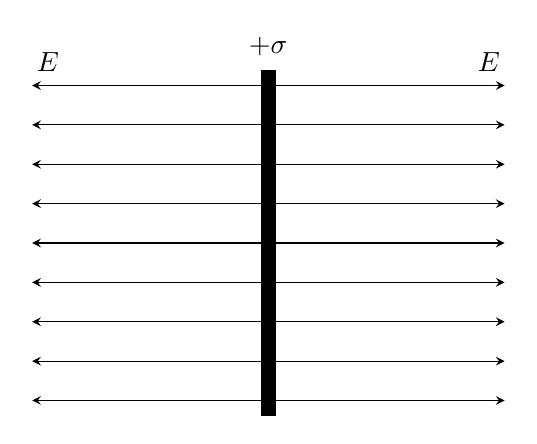
\begin{tikzpicture}[>=stealth,scale=1.0]
                        \fill [black] (-0.1,2.2) rectangle (0.1,-2.2);
                        \node at(0,2.5) {$+\sigma$};
        
                        \draw[->] (0.1,2.0)--(3,2.0);
                        \draw[->] (0.1,1.5)--(3,1.5);
                        \draw[->] (0.1,1.0)--(3,1.0);
                        \draw[->] (0.1,0.5)--(3,0.5);
                        \draw[->] (0.1,0.0)--(3,0.0);
                        \draw[->] (0.1,-0.5)--(3,-0.5);
                        \draw[->] (0.1,-1.0)--(3,-1.0);
                        \draw[->] (0.1,-1.5)--(3,-1.5);
                        \draw[->] (0.1,-2.0)--(3,-2.0);
        
                        \draw[->] (-0.1,2.0)--(-3,2.0);
                        \draw[->] (-0.1,1.5)--(-3,1.5);
                        \draw[->] (-0.1,1.0)--(-3,1.0);
                        \draw[->] (-0.1,0.5)--(-3,0.5);
                        \draw[->] (-0.1,0.0)--(-3,0.0);
                        \draw[->] (-0.1,-0.5)--(-3,-0.5);
                        \draw[->] (-0.1,-1.0)--(-3,-1.0);
                        \draw[->] (-0.1,-1.5)--(-3,-1.5);
                        \draw[->] (-0.1,-2.0)--(-3,-2.0);
                        
                        \node at(-2.8,2.3) {$E$};
                        \node at(2.8,2.3) {$E$};
                    \end{tikzpicture}
                    \caption{一块无限大均匀带电平面[正电]}
                \end{minipage}
            }\qquad\qquad
            \subfigure
            {
                \begin{minipage}[t]{0.4\linewidth}
                    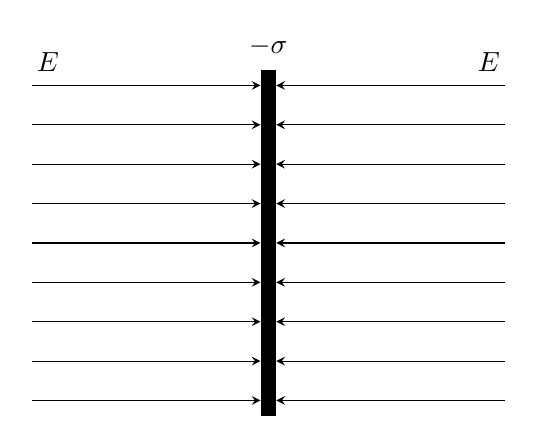
\begin{tikzpicture}[>=stealth,scale=1.0]
                        \fill [black] (-0.1,2.2) rectangle (0.1,-2.2);
                        \node at(0,2.5) {$-\sigma$};
        
                        \draw[->] (3,2.0)--(0.1,2.0);
                        \draw[->] (3,1.5)--(0.1,1.5);
                        \draw[->] (3,1.0)--(0.1,1.0);
                        \draw[->] (3,0.5)--(0.1,0.5);
                        \draw[->] (3,0.0)--(0.1,0.0);
                        \draw[->] (3,-0.5)--(0.1,-0.5);
                        \draw[->] (3,-1.0)--(0.1,-1.0);
                        \draw[->] (3,-1.5)--(0.1,-1.5);
                        \draw[->] (3,-2.0)--(0.1,-2.0);
        
                        \draw[->] (-3,2.0)--(-0.1,2.0);
                        \draw[->] (-3,1.5)--(-0.1,1.5);
                        \draw[->] (-3,1.0)--(-0.1,1.0);
                        \draw[->] (-3,0.5)--(-0.1,0.5);
                        \draw[->] (-3,0.0)--(-0.1,0.0);
                        \draw[->] (-3,-0.5)--(-0.1,-0.5);
                        \draw[->] (-3,-1.0)--(-0.1,-1.0);
                        \draw[->] (-3,-1.5)--(-0.1,-1.5);
                        \draw[->] (-3,-2.0)--(-0.1,-2.0);
                        
                        \node at(-2.8,2.3) {$E$};
                        \node at(2.8,2.3) {$E$};
                    \end{tikzpicture}
                    \caption{一块无限大均匀带电平面[负电]}
                \end{minipage}
            }
        \end{center}
    \end{figure}\\
    我们取闭合圆柱面为高斯面,圆柱体底面与带电平面平行,圆柱体侧面与带电平面垂直。\\[3mm]
    设圆柱体的长为$2r$,设圆柱体的底面积为$S$,设圆柱体的底面场强为$E$。\\[3mm]
    由于圆柱侧面与电场线平行,电通量为$0$。\\[3mm]
    由于圆柱底面与电场线垂直,电通量为$\Phi$。\\[5mm]
    根据高斯电场定律:
    \setcounter{equation}{0}
    \begin{align}
        &\Phi=\frac{1}{\varepsilon_0}\cdot Q\\[3mm]
        &2\cdot E\cdot S=\frac{1}{\varepsilon_0}\cdot\sigma\cdot S\\[3mm]
        &2\cdot E=\frac{1}{\varepsilon_0}\cdot\sigma\\[3mm]
        &E=\frac{\sigma}{2\cdot\varepsilon_0}
    \end{align}\\
    由此可见,一块无限大均匀带电平面周围的电场是和距离无关的匀强电场。\\[3mm]
    一块无限大均强电平面周围的电场强度公式:
    \begin{large}
        \begin{equation*}
            E=\frac{\sigma}{2\cdot\varepsilon_0}
        \end{equation*}
    \end{large}

\newpage

    类似的,我们也可以由此得出另外一种匀强电场。\\[3mm]
    设两块无限大均匀带电平面,设带电平面上单位面积上带有的电荷量分别为$\pm\sigma$。\\[3mm]
    根据上方的结论,对于平面间的区域,两者场强叠加,对于平面外的区域,两者场强抵消。\\[3mm]
    根据上述设定,我们有以下示意图:
    \begin{figure}[h]
        \begin{center}
            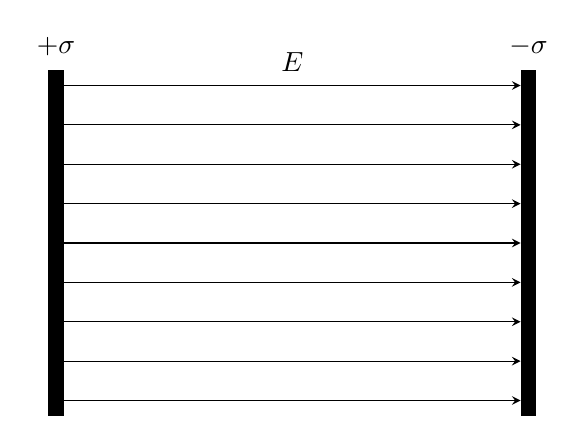
\begin{tikzpicture}[>=stealth,scale=1.0]
                \fill [black] (-3.1,2.2) rectangle (-2.9,-2.2);
                \node at(-3,2.5) {$+\sigma$};
                \fill [black] (2.9,2.2) rectangle (3.1,-2.2);
                \node at(3,2.5) {$-\sigma$};

                \draw[->] (-2.9,2.0)--(2.9,2.0);
                \draw[->] (-2.9,1.5)--(2.9,1.5);
                \draw[->] (-2.9,1.0)--(2.9,1.0);
                \draw[->] (-2.9,0.5)--(2.9,0.5);
                \draw[->] (-2.9,0.0)--(2.9,0.0);
                \draw[->] (-2.9,-0.5)--(2.9,-0.5);
                \draw[->] (-2.9,-1.0)--(2.9,-1.0);
                \draw[->] (-2.9,-1.5)--(2.9,-1.5);
                \draw[->] (-2.9,-2.0)--(2.9,-2.0);

                \node at(0,2.3) {$E$};
            \end{tikzpicture}
            \caption{两块无限大均匀带电平面}
        \end{center}
    \end{figure}\\
    根据场强叠加定理:
    \setcounter{equation}{0}
    \begin{align}
        &E=E^++E^-\\[3mm]
        &E=\frac{\sigma}{2\cdot\varepsilon_0}+\frac{\sigma}{2\cdot\varepsilon_0}\\[3mm]
        &E=\frac{\sigma}{\varepsilon_0}
    \end{align}\\
    由此可见,两块无限大均匀带电平面之间的电场是和距离无关的匀强电场。\\[3mm]
    两块无限大均强电平面之间的电场强度公式:
    \begin{large}
        \begin{equation*}
            E=\frac{\sigma}{\varepsilon_0}
        \end{equation*}
    \end{large}

\newpage

\section{电路}

\subsection{电流}
    电流衡量了单位时间内通过的电荷量。\\[4mm]
    电流符号:$I$\\[1mm]
    电流单位:A~~安培\\[4mm]
    电流单位安培的定义:A $=$ C / s\\[1mm]
    在$1$秒内流过$1$库伦的电荷称为$1$安培。\\[3mm]
    电流的宏观表达式:
    \begin{large}
        \begin{equation*}
            I=\frac{Q}{t}
        \end{equation*}
    \end{large}\\
    我们也可以从微观角度理解电流:\\[3mm]
    1.导体横截面的面积是$S$\\[2mm]
    2.自由电荷的电荷量是$q$\\[2mm]
    3.自由电荷的速度是$v$\\[2mm]
    4.单位体积内导体中自由电荷的数量为$n$\\[5mm]
    显然在时间$\Delta t$中,体积$S\cdot v\cdot\Delta t$内的自由电荷全部通过了横截面:\vspace{8pt}
    \setcounter{equation}{0}
    \begin{align}
        I=\frac{Q}{\Delta t}=\frac{(S\cdot v\cdot \Delta t)\cdot(n\cdot q)}{\Delta t}
    \end{align}\\
    电流的微观表达式:
    \begin{large}
        \begin{equation*}
            I=n\cdot q\cdot S\cdot v
        \end{equation*}
    \end{large}

\subsection{电压}
    电压衡量了两个位置间的电势差。\\[4mm]
    电压符号:$U$\\[1mm]
    电压单位:V~~伏特\\[4mm]
    电压单位伏特的定义:V $=$ J / C\\[1mm]
    在电场中两点电势差为$1$~J/C时称为$1$伏特。

\newpage

\subsection{电阻}
    电阻符号:$R$\\[1mm]
    电阻单位:$\Omega$~~欧姆\\[4mm]
    电阻单位欧姆的定义:$\Omega=$ V / A\\[1mm]
    通过$1$安培的电流需要施加$1$伏特的电压,
    我们认为这个电阻具有$1$欧姆。\\[3mm]
    电阻代表了对电流的阻抗程度,
    电阻越大,代表通过相同的电流所需要施加的电压越大,
    欧姆定律定理的描述了电阻和电流电压的关系。\\[3mm]
    欧姆定律:
    \begin{large}
        \begin{equation*}
            R=\frac{U}{I}
        \end{equation*}
    \end{large}
    
\subsubsection{电阻定律}
    我们可以通过电阻率来比较材料导电性能的强弱。\\[3mm]
    电阻率符号:$\rho$\\
    电阻率单位:$\Omega \cdot\text{m}$\\[3mm]
    电阻率单位的定义:$\Omega \cdot \text{m}=\Omega \cdot \dfrac{\text{m}^2}{\text{m}}$\\[3mm]
    电阻率衡量了单位截面积的某种导体,
    在单位长度下的阻值。\\[3mm]
    在温度一定时,电阻的阻值满足公式:
    \begin{large}
        \begin{equation*}
            R = \rho \cdot \dfrac{l}{S}       
        \end{equation*}
    \end{large}\\[3mm]
    这个公式被称为电阻定律,由此我们可以得出结论:
    对于特定某种导体,在温度一定时,
    阻值和电阻长度成正比,而和电阻的横截面积成反比。\\[3mm]
    对于电阻和长度的关系,我们可以这样理解,电阻的本质是材料对于电子的阻抗作用,
    显然穿过一个长度为$2l$的导体所受到的阻抗是长度为$l$的导体的两倍。\\[3mm]
    对于电阻和截面积的关系,我们可以这样理解,
    在电压相同的前提下,当截面积为$S$时,
    只能容纳一个电子通过,
    而当截面积为$2S$时,显然就可以通过两个电子,
    可以看出后者的电流是前者的两倍,
    根据欧姆定律,我们可以发现后者的电阻只有前者的一半。

\newpage

\subsection{电池}
    电池的本质是这样的:电子从电势较高的一端流出,
    流到电势较低的一端,显然这个过程需要释放能量,
    而这部分能量便是为我们所用,用于驱动用电器,
    这个过程也可以这样理解,
    能量较高的电子流经用电器时释放出了其所携带的能量,
    变成了能量较低的电子。\\[3mm]
    那么电池的意义究竟在哪里?\\[3mm]
    显然那部分流到电势较低的电子
    不会自发的移动到电势较高的位置,
    或者说能量较低的电子显然也不会自发的吸收
    能量成为能量较高的电子。\\[3mm]
    储存的大量的能量较高的电子显然是非常困难,
    所以我们需要通过某种方式,循环的
    为能量较低的电子补充能量,
    使其重新成为能量较高的电子。\\[3mm]
    也就是说我们需要通过外力做功,
    将电子从电势较低处移到电势较高处。\\[3mm]
    这便是电池的意义所在,电池储存了大量化学物质,
    这些化学物质可以通过反应,通过“化学力”达到对电子做功的目的。
    电池通过这些储能效率高化学物质,利用化学反应
    将化学物质内储存的化学能持续的转化为电能。
    从而可以得到一个稳定的电压,以此来维持电路中电流的稳定。\\[3mm]
    对于不可充电的电池,电池内的化学物质的反应大多是单向的,
    当电池耗尽反应物时,电池便会无法维持电压,
    此时我们通常就会说这个电池没电了。\\[3mm]
    对于可反复充电的电池,电池内的化学物质的反应可以是双向的,
    既正向反应可以对电子做功,将其从低电势转移到高电势,
    但当将电池作为用电器时,通过能量高的电子所释放的能量,
    可以促使反应逆向进行,使低能的产物重新变成高能的反应物,
    从而实现可以反复的充电放电。\\

\subsubsection{电池的结构}
    从电池外部看,电势从负极至正极升高,
    但实际上,在电池的内部,某些地方的电势会升高,
    某些地方的电势会降低,
    我们可以通过化学上的原电池来研究电池内部的电势变化。\\[3mm]
    在电池的正极和负极处,化学力做正功,电势升高,
    这是由于电池的两极是和溶液发生化学反应的位置,
    化学能被消耗,从而使电势升高。\\[3mm]
    在电池内部的电解液中,电场力做正功,电势降低,
    这是由于电解液对在两极间移动的离子有阻碍作用,
    电势能被消耗,从而使电势降低。\\[3mm]
    电池的电解液所产生的电阻称为内电阻。

\newpage

\subsection{电动势}
    电动势衡量了一个电池将电荷从负极搬运至正极的能力强弱,
    换言之,电动势指的就是电势在电池的两极处所升高的值。
    电动势是电源自身的一个属性,只取决与电池本身的结构。\\[3mm]
    虽然电动势和电压的单位相同,均为伏特,但两者的意义是相反的:\\[3mm]
    电压衡量了$1$库伦的电荷流过电路时,有多少焦耳的能量由电能转化为其他形式。\\[1mm]
    电动势衡量了$1$库伦的电荷流过电源时,有多少焦耳的能量由其他形式转化为电能。\\[3mm]
    电动势实际上代表了一个电池理论上可以输出的最大电压,
    但是由于电池必然有一定的内阻,会夺取一部分电压,
    所以电池实际输出的电压必然小于电动势。\\[3mm]
    电动势通常使用符号$E$或符号$\mathscr{E}$表示。

\subsection{闭合电路}
    我们将电源外部,从正极至负极的部分称为外电路。\\[1mm]
    我们将电源内部,从负极至正极的部分称为内电路。\\[3mm]
    我们将内电路和外电路合称为闭合电路,在初中阶段,
    由于我们不需要考虑电池的内阻,
    也就是忽略了内电路的影响,
    所以实际上研究的只是闭合电路中的外电路。\\[3mm]
    当我们考虑内电阻的影响时,通过欧姆定律可以推导出如下公式:\\[3mm]
    电流等于电动势除以内外阻值之和:
    \begin{large}
        \begin{equation*}
            I = \frac{E}{R+r}       
        \end{equation*}
    \end{large}\\
    电动势等于电流乘以内外阻值之和:
    \begin{large}
        \begin{equation*}
            E = I \cdot \left(R+r\right)
        \end{equation*}
    \end{large}

\newpage

\subsection{内电阻的测量}
    首先,内电阻并非真正意义上的电阻,所以显然我们不能直接的进行测量。\\[3mm]    
    第一步,我们将电池接在电压表两端,
    由于电压表的电阻值趋向于无穷大,依照极限的思想,
    内电压趋向于零,外电压趋向于电动势,
    所以此时测得的电压就是电动势的大小。\\[3mm]
    第二步,我们将电池接在电流表两端
    由于电流表的电阻值趋向于无穷小,依照极限的思想,
    外电阻趋向于零,此时电路中唯一的负载是电池内阻,
    所以此时测得的电流就是电源的短路电流。\\[3mm]
    由此我们得到了电源的电动势和短路电流,
    根据欧姆定律计算即可得到内电阻,
    但是这样的方法存在一个问题,
    需要将电池短路来测得电流,
    然而短路这样的操作终究会对电池造成损害,
    过于野蛮,所以接下来我们再提出一种更加文明的方式。\\[3mm]
    将电路中接入一个滑动变阻器,
    将滑动变阻器移到不同位置,
    测得两组电流电压。\\[3mm]
    建立以下方程组:
    \begin{large}
        \begin{equation*}
            \begin{cases}
                \ E=U_{1}+I_{1} \cdot r\\[1mm]
                \ E=U_{2}+I_{2} \cdot r \vspace{3pt}               
            \end{cases}
        \end{equation*}
    \end{large}\\
    经过化解后可得:
    \begin{large}
        \begin{equation*}
            r=\dfrac{U_{1}-U_{2}}{I_{2}-I_{1}}
        \end{equation*}
    \end{large}\\
    由此可以在保证电池安全的情况下测得电源内阻。

\newpage

\subsection{串联}
    \begin{figure}[h!]
        \begin{center}
            \begin{circuitikz}[european resistors]
            \draw (-4,0)
            to[short] (-3,0)
            to[R=$R_1$] (-1,0)
            to[short] (1,0)
            to[R=$R_2$] (3,0)
            to[short] (4,0);
            \end{circuitikz}
            \caption{串联电路示意图}
        \end{center}
    \end{figure}

    我们可以认为串联电路就是将若干个电阻拼接为一个长度更长的电阻,
    由于阻值和电阻长度成正比,
    所以串联电路的总阻值等于各个电阻的阻值和。\\[3mm]
    串联电路的特点:电流处处相等,
    电压之比等于电阻之比,
    总电阻等于各个电阻的阻值和,
    总电压等于各个电阻的电压和。\\[3mm]
    所以我们可以用如下公式描述串联电路中的物理量:\\[3mm]
    电压之比等于电阻之比:
    \begin{large}
        \begin{equation*}
            U_1:U_2=R_1:R_2
        \end{equation*}
    \end{large}\\[3mm]
    总电阻等于各个电阻的阻值和:
    \begin{large}
        \begin{equation*}
            R=R_1+R_2+\hdots+R_n       
        \end{equation*}
    \end{large}\\[3mm]
    总电压等于各个电压的阻值和:
    \begin{large}
        \begin{equation*}
            U=U_1+U_2+\hdots+U_n
        \end{equation*}
    \end{large}\\[3mm]

\newpage

\subsection{并联}
    \begin{figure}[h!]
        \begin{center}
            \begin{circuitikz}[european resistors]
            \draw (-4,0)
            to[short] (-2,0);
            \draw (-2,0)
            to[short] (-2,1)
            to[short] (-1,1)
            to[R=$R_1$] (1,1)
            to[short] (2,1)
            to[short] (2,0);
            \draw (-2,0)
            to[short] (-2,-1)
            to[short] (-1,-1)
            to[R=$R_2$] (1,-1)
            to[short] (2,-1)
            to[short] (2,0);
            \draw (2,0)
            to[short] (4,0);
            \end{circuitikz}
            \caption{并联电路示意图}
        \end{center}
    \end{figure}
    我们可以认为并联电路就是将若干个电阻拼接为一个横截面积更大的电阻,
    由于阻值和横截面积成反比,所以并联电路的总电阻等于各个电阻阻值的倒数和的倒数。\\[3mm]
    并联电路的特点:
    电压处处相等,电流之比等于电阻之反比,
    总电阻等于各个电阻阻值的倒数和的倒数,
    总电流等于各个电阻的电流和。\\[3mm]
    所以我们可以用如下公式描述并联电路中的物理量:\\[3mm]
    电流之比等于电阻之反比:
    \begin{large}
        \begin{equation*}
            I_1:I_2=\frac{1}{R_1}:\frac{1}{R_2}
        \end{equation*}
    \end{large}\\[1mm]
    总电阻等于各个电阻阻值的倒数和的倒数:
    \begin{large}
        \begin{equation*}
            R=\frac{1}{\frac{1}{R_1}+\frac{1}{R_2}+\hdots+\frac{1}{R_n}}
        \end{equation*}
    \end{large}\\[1mm]
    总电流等于各个电阻的电流和:
    \begin{large}
        \begin{equation*}
            I=I_1+I_2+\hdots+I_n
        \end{equation*}
    \end{large}\\[1mm]
    特别的,当电路中只有两个电阻时:
    \begin{large}
        \begin{equation*}
            R=\frac{R_1 \cdot R_2}{R_1+R_2}
        \end{equation*}
    \end{large}\\[1mm]
    特别的,当电路中的电阻阻值都相同时:
    \begin{large}
        \begin{equation*}
            R=\frac{R_0}{n}
        \end{equation*}
    \end{large}\\[1mm]
    并联电阻的总阻值一定小于任何一个电阻的阻值。
    当两个电阻并联时,
    若其中一个电阻的的阻值远远大于另一个,
    那么总阻值会无限接近于阻值较小的电阻。

\newpage

\subsection{基尔霍夫定律}
    基尔霍夫定律描述了电路中电流和电压所遵循的基本规律,可以用于对复杂电路的分析和计算。

\subsubsection{电流节点定律}
    电流节点定律(基尔霍夫第一定律):任何一个节点,流入电流的总和等于流出电流的总和。\\[3mm]
    根据电流节点定律,我们可以列出若干电流节点方程,组成的方程组称为基尔霍夫第一方程组。\\[3mm]
    在使用电流节点定律时,各个支路的电流方向可以任意设定,
    但一旦设定方向,所有电流节点方程都必须依照所设定的电流方向构造,
    不得再随意变换。\\[3mm]
    若电流真实方向与设定方向相同,解出的电流值为正。\\[2mm]
    若电流真实方向与设定方向相反,解出的电流值为负。\\[3mm]
    通常情况下我们应当将电流方向设定为其真实方向,
    但对于一部分复杂的电路,其中可能有若干支路的电流方向是无法确定,
    这种情况下可以先随意的设定一个方向列出方程,
    求解后根据电流的正负判断其真实方向。\\[3mm]
    在列电流节点方程时需要注意,
    如果一个电路中有$n$个节点,那么只能列$n-1$个方程,
    多余的方程仍然成立,但必然和已列出的方程等价。

\subsubsection{电压回路定律}
    电压回路定律(基尔霍夫第二定律):任何一个回路,绕其一圈的电压和为零。\\[3mm]
    根据电压节点定律,我们可以列出若干电压回路方程,组成的方程组称为基尔霍夫第二方程组。\\[3mm]
    使用电压回路定律时,可以从电路中任意一点开始,
    沿着电路每遇到一个元件,按照以下规则进行电压的升降,
    最终回到该点时,电压为零。\\[3mm]
    从电源正极到负极电压降$U$。\\[2mm]
    从电源负极到正极电压升$U$。\\[2mm]
    顺电流方向遇到一个电阻电压降$R\cdot I$。\\[2mm]
    逆电流方向遇到一个电阻电压升$R\cdot I$。\\[2mm]
    电源内阻作为一般电阻处理即可。\\[3mm]
    在列电压回路方程时需要注意,
    在每列出一个新的方程时,
    需要确保回路中至少有一段电路是之前的方程中从未使用过的,
    多余的方程仍然成立,但必然和已列出的方程等价。

\subsubsection{具体应用方法}
    联立基尔霍夫第一方程组和基尔霍夫第二方程组,
    通过电流节点方程代换电压回路方程中的未知量,
    减少未知量,最终会得到一个多元一次方程组,
    求解即可得到答案。

\newpage

\subsection{戴维宁定律}
    戴维宁定律提出了一种使用等效电源替代部分电路的方法,可以有效简化复杂电路。\\[3mm]
    戴维宁定律:对于一个两端电路,可以将其等效为由一个电压源和一个电阻串联成的两端电路,
    电压等于两端电路的开路电压,电阻等于两端电路在所有电压源被短路时的等效电阻。\\[3mm]
    例如我们可以使用右图的电路等效左图的电路:\vspace{8pt}
    \begin{figure}[h]
        \begin{center}
            \subfigure[原始电路]
            {
                \begin{minipage}[t]{0.33\linewidth}
                    \begin{circuitikz}[european resistors]
                        \draw (-2.5,0) to[battery1] (0,0);
                        \draw (0,0) to[generic] (2.5,0);
                        \draw (-2.5,0) to[short] (-2.5,3);
                        \draw (2.5,0) to[short] (2.5,3);
                        \draw (-2.5,1) to[generic] (2.5,1);
                        \draw (-2.5,2) to[generic] (2.5,2);
                        \draw (-2.5,3) to[short,-o] (-1,3);
                        \draw (2.5,3) to[short,-o] (1,3);
                    \end{circuitikz}
                \end{minipage}
            }\qquad\qquad
            \subfigure[等效电路]
            {
                \begin{minipage}[t]{0.33\linewidth}
                    \begin{circuitikz}[european resistors]
                        \draw (-2.5,0) to[battery1] (0,0);
                        \draw (0,0) to[generic] (2.5,0);
                        \draw (-2.5,0) to[short] (-2.5,2);
                        \draw (2.5,0) to[short] (2.5,2);
                        \draw (-2.5,2) to[short,-o] (-1,2);
                        \draw (2.5,2) to[short,-o] (1,2);
                    \end{circuitikz}
                \end{minipage}
            }
            \caption{戴维宁定律示意图}
        \end{center}
    \end{figure}\\
    在计算等效电路的电压时,可以在原始电路中接入:
    \begin{figure}[h]
        \begin{center}
            \begin{circuitikz}[european resistors]
                \draw (-3,0) to[voltmeter] (3,0);
            \end{circuitikz}
            \caption{等效电路电压的计算}
        \end{center}
    \end{figure}\\
    在计算等效电路的电阻值时,可以在原始电路中接入:
    \begin{figure}[h]
        \begin{center}
            \begin{circuitikz}[european resistors]
                \draw (-3,0) to[battery1] (0,0);
                \draw (0,0) to[ammeter] (3,0);
            \end{circuitikz}
            \caption{等效电路电流的计算}
        \end{center}
    \end{figure}\\
    设电压表的读数为$U_V$,那么等效电源的电压$U$:
    \begin{large}
        \begin{equation*}
            U=U_V
        \end{equation*}
    \end{large}\\
    设电流表的读数为$I_A$,那么等效电源的电阻$R$:\vspace{8pt}
    \begin{large}
        \begin{equation*}
            R=\frac{U}{I_A}
        \end{equation*}
    \end{large}

\newpage

\subsection{电功率}
    电功率衡量了单位时间内消耗的电能大小。\\[4mm]
    电功率符号:$P$\\[1mm]
    电功率单位:W~~瓦特\\[4mm]
    电功率单位瓦特的定义:W $=$ V $\cdot$ A\\[1mm]
    在电路中,若电压为1伏特,电流为1安培,那么此时的电功率为1瓦特。\\[5mm]
    电流代表了单位时间内通过的电荷量,
    电压代表了单位电荷量所具有的能量,
    很显然两者的积就是电功率,
    由此我们可以得出电功率的计算公式。\\[3mm]
    电功率的计算公式:
    \begin{large}
        \begin{equation*}
            P=U\cdot I
        \end{equation*}
    \end{large}\vspace{-10pt}

\subsection{电功}
    电功衡量了电流做功的多少。\\[3mm]
    电功的计算公式:
    \begin{large}
        \begin{equation*}
            W=U\cdot I\cdot t
        \end{equation*}
    \end{large}\\
    电热衡量了电流做功产生热量的多少。\\[3mm]
    电热的计算公式:
    \begin{large}
        \begin{equation*}
            Q=I^2\cdot R\cdot t
        \end{equation*}
    \end{large}\\
    对于纯电阻电路,所有电能均被电阻消耗,转化为热量,
    所以这种情况下电功等于电热。\\[3mm]
    对于非纯电阻电路,部分电能被电阻消耗,转化为热量,
    大部分电能通过电流做功转化为其他形式的能量,
    所以这种情况下电功大于电热。\\[3mm]
    电热的计算公式也被称为焦耳定律。\\[3mm]
    电功的单位是焦耳,但这个单位并不利于使用,
    所以我们通常会使用千瓦时来衡量电功的大小,
    1千瓦时代表了电路以1千瓦的电功率工作一个小时所做的功。\\[3mm]
    在日常生活中,我们通常也将千瓦时称为度。

\newpage

\section{磁场}

\subsection{磁场力}
    磁场力是由于电流而产生的力,指的是两个电流元间通过磁场产生的力。\\[2mm]
    磁场力与距离的平方成反比,与电流之积成正比。\\[3mm]
    磁场力公式:
    \begin{large}
        \begin{equation*}
            \dif F=k\cdot\frac{I_1 \cdot I_2}{r^2}\cdot \dif l^2\cdot\sin{\alpha}\cdot\sin{\beta}
        \end{equation*}
    \end{large}\\
    其中k为磁场力公式的比例系数:
    \begin{large}
        \begin{equation*}
            k=1.0\times 10^{-7}~\text{N / A}^2
        \end{equation*}
    \end{large}\\
    磁场力公式的比例系数$k$可以通过真空磁导率$\mu_0$推导:
    \begin{large}
        \begin{equation*}
            k=\dfrac{\mu_0}{4\cdot\pi}
        \end{equation*}
    \end{large}\\
    磁场力公式是由安培发现的,所以该公式也被称为安培定律,而磁场力有时也被称为安培力。\\[3mm]
    为了纪念安培做出的伟大贡献,我们用安培命名电流的单位。\\

\subsection{磁感强度}
    磁感强度描述了磁场的强弱,代表了具有单位电流的电流元在磁场中受到的磁场力。\\[1mm]
    磁感强度与距离的平方成反比,与电流成正比。\\[3mm]
    磁感强度公式:
    \begin{large}
        \begin{equation*}
            \dif B = \dfrac{k \cdot I_{1}}{{r}^{2}}\cdot \dif l\cdot\sin{\alpha}
        \end{equation*}
    \end{large}\\
    磁感强度单位:N / A $\cdot$ m\\[3mm]
    为了纪念美国电气技师特斯拉,我们用特斯拉($T$)命名磁感强度单位。\\[6mm]
    这个结论也被称为毕奥-萨伐尔定律。

\newpage

\subsection{关于磁场力和磁感强度的说明}
    上述表述中,提到了电流元的概念,
    电流元实际指的是一段无穷短的通电导线,其长度为$\dif l$。\\[3mm]
    通过电流元的概念,我们得以对“磁场中的电流元”和“电场中的电荷”这两者进行类比,
    从而更好的认识电和磁的相似之处。
    虽然电流元这样无穷短的通电导线并不存在于现实中,
    但是其清楚的揭示了磁场的本质规律,
    同时我们也可以通过积分的方式,
    得到诸如通电长直导线等宏观物体所产生磁场的性质。\\[3mm]
    考虑以下示意图:
    \begin{figure}[h]
        \begin{center}
            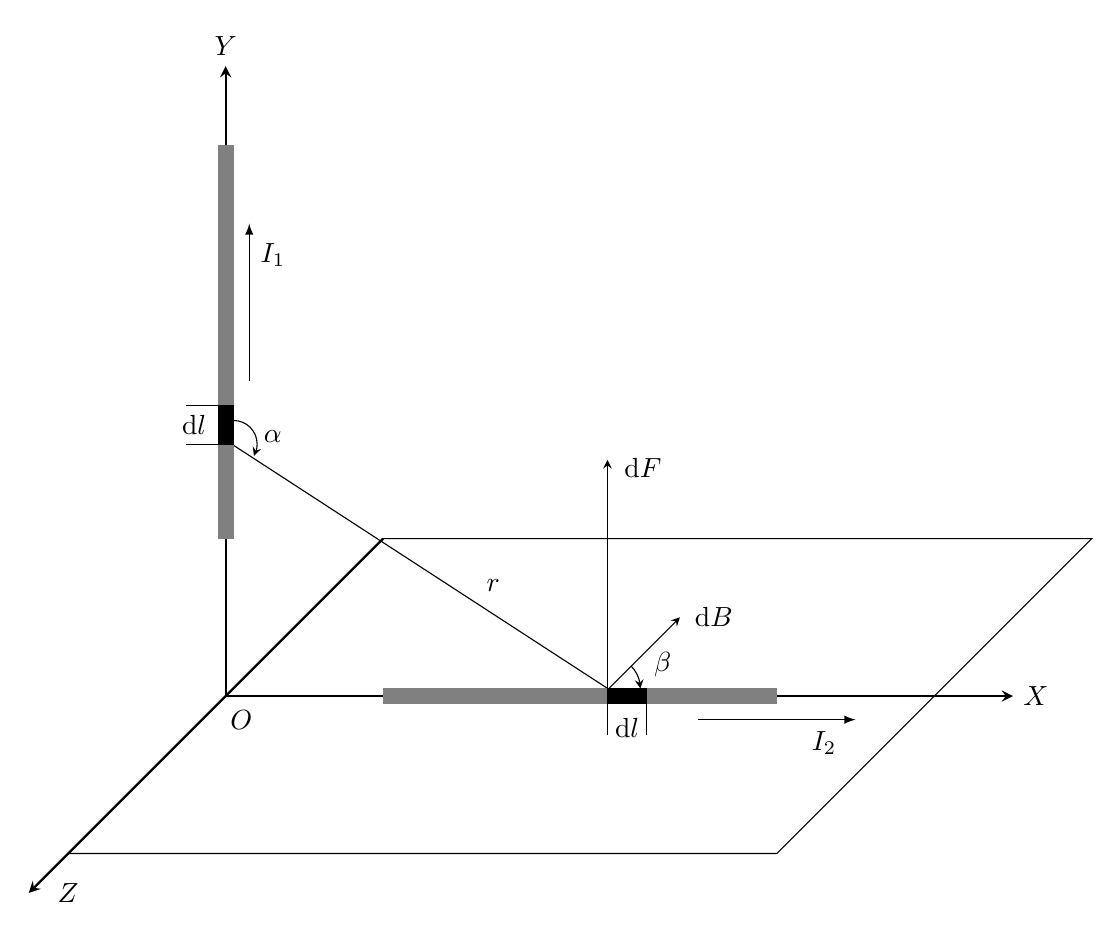
\begin{tikzpicture}[>=stealth,scale=1.0]
                \draw[->,thick](0,0)--(10,0) node[right] {$X$};
                \draw[->,thick](0,0)--(0,8) node[above] {$Y$};
                \draw[->,>=stealth,thick](2,2)--(-2.5,-2.5) node at(-2,-2.5) {$Z$};
                \draw[-](2,2)--(11,2)--(7,-2)--(-2,-2);
            
                \node at(0.2,-0.3) {$O$};        
                \draw [->,>=stealth](4.77,0)--(5.77,1) node at(6.2,1) {$\dif B$};
                \draw [->,>=stealth](4.85,0)--(4.85,3) node at(5.3,2.9) {$\dif F$};
                \draw [-](5,0)--(0,3.25);
                \node at(3.4,1.4) {$r$};
                \draw [->,>=stealth](0.1,3.5) arc(90:-30:0.3);
                \node at(0.6,3.3) {$\alpha$};
                \draw [->,>=stealth](5.15,0.38) arc(45:0:0.4);
                \node at(5.55,0.4) {$\beta$};

                \fill [gray] (-0.1,2) rectangle (0.1,7);
                \fill [black] (-0.1,3.19) rectangle (0.1,3.69);
                \draw [-latex] (0.3,4)--(0.3,6);
                \node at(0.6,5.6) {$I_1$};

                \fill [gray] (2,-0.1) rectangle (7,0.1);
                \fill [black] (4.85,-0.1) rectangle (5.35,0.1);
                \draw [-latex] (6,-0.3)--(8,-0.3);
                \node at(7.6,-0.6) {$I_2$};

                \draw[-] (0.1,3.19)--(-0.5,3.19);
                \draw[-] (0.1,3.69)--(-0.5,3.69);
                \node at(-0.4,3.45) {$\dif l$};

                \draw[-] (4.85,0.1)--(4.85,-0.5);
                \draw[-] (5.35,0.1)--(5.35,-0.5);
                \node at(5.10,-0.4) {$\dif l$};
            \end{tikzpicture}
            \caption{磁感强度和磁场力的示意图}
        \end{center}        
    \end{figure}\\
    磁感强度的方向始终垂直于由电流元$I_1$与$r$构成的平面,具体使用右手螺旋定则判定。\\[2mm]
    \textbf{右手螺旋定则:}
    用右手握住电流元,拇指指向电流的方向,
    四指指向磁感强度的方向。\\[4mm]
    磁场力的方向始终垂直于由电流元$I_2$与$\dif B\:$构成的平面,具体使用左手定则判定。\\[2mm]
    \textbf{左手定则:}
    伸开左手,
    使得磁感强度在垂直于导线上的分量从手心方向垂直刺入,这种情况下,
    四指指向电流的方向,拇指指向磁场力的方向。

\newpage

\subsection{通电直导线产生的磁场作用}
    如图,对于一条通电直导线,
    我们需要计算其附近任意一点$P$处的磁感强度。\\[3mm]
    我们可以利用毕奥-萨伐尔定律,
    首先得出通电直导线上的电流元在$P$处产生的磁感强度,
    并对其积分,从而得到通电直导线在$P$点的磁感强度。\\[1mm]
    \begin{figure}[h]
        \begin{center}
            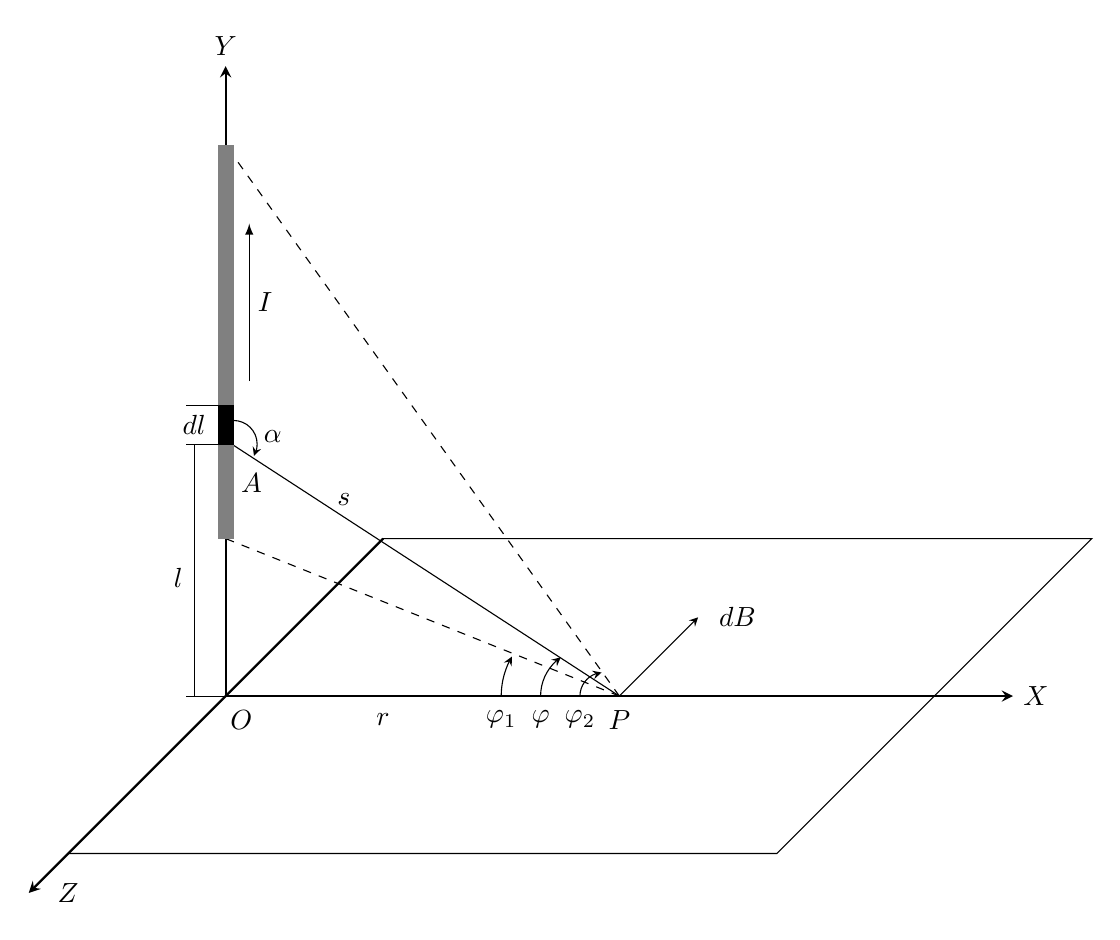
\begin{tikzpicture}[>=stealth,scale=1.0]
                \draw[->,thick](0,0)--(10,0) node[right] {$X$};
                \draw[->,thick](0,0)--(0,8) node[above] {$Y$};
                \draw[->,>=stealth,thick](2,2)--(-2.5,-2.5) node at(-2,-2.5) {$Z$};
                \draw[-](2,2)--(11,2)--(7,-2)--(-2,-2);
            
                \node at(0.2,-0.3) {$O$};        
                \node at(5,-0.3) {$P$};
                \node at(2,-0.3) {$r$};
                \draw [->,>=stealth](5,0)--(6,1) node at(6.5,1) {$dB$};
                \draw [dashed](5,0)--(0,7);
                \draw [dashed](5,0)--(0,2);
                \draw [-](5,0)--(0,3.25);
                \node at(1.5,2.5) {$s$};
                \draw [->,>=stealth](0.1,3.5) arc(90:-30:0.3);
                \node at(0.6,3.3) {$\alpha$};
                \draw [->,>=stealth](4.5,0) arc(180:95:0.3);
                \node at(4.5,-0.3) {$\varphi_2$};
                \draw [->,>=stealth](4,0) arc(180:125:0.6);
                \node at(4.05,-0.3) {$\varphi_{\;}$};
                \draw [->,>=stealth](3.5,0) arc(180:150:1.0);
                \node at(3.5,-0.3) {$\varphi_1$};

                \fill [gray] (-0.1,2) rectangle (0.1,7);
                \fill [black] (-0.1,3.19) rectangle (0.1,3.69);
                \draw [-latex] (0.3,4)--(0.3,6);
                \node at(0.5,5) {$I$};

                \draw[-] (0.1,3.19)--(-0.5,3.19);
                \draw[-] (0.1,3.69)--(-0.5,3.69);
                \node at(-0.4,3.45) {$dl$};

                \draw[-] (0.1,0)--(-0.5,0);            
                \draw[-](-0.4,3.19)--(-0.4,0);
                \node at(-0.6,1.5) {$l$};

                \node at(0.33,2.7) {$A$};
            \end{tikzpicture}
            \caption{通电直导线产生的磁场作用}
        \end{center}        
    \end{figure}\\
    根据毕奥-萨伐尔定律:\vspace{3pt}
    \setcounter{equation}{0}
    \begin{equation}
        \dif B=\frac{k\cdot I}{s^2}\cdot\dif l\cdot\sin{\alpha}
    \end{equation}\\
    由于我们考虑的是通电直导线,
    所以导线上各个电流元在点$P$处产生的磁感强度的方向是一致的,
    通过积分可以得到点$P$处的总磁感强度:\vspace{5pt}
    \begin{equation}
        B=\int_{L}\dif B=\int_{L} \frac{k\cdot I}{s^2}\cdot\dif l\cdot\sin{\alpha}
    \end{equation}\\
    为了便于积分,我们需要使用一个统一的参数进行变量替换,我们不妨设:
    \begin{equation}
        \varphi=\angle{APO}
    \end{equation}

\newpage

    使用参数$\varphi$替换变量:
    \begin{align}
        &\sin{\alpha}=\cos{\varphi}\\[3mm]
        &~s=r\cdot\sec{\varphi}\\[3mm]
        &~l\;=r\cdot\tan{\varphi}\\[3mm]
    \end{align}
    求$l$的微分$dl$:
    \begin{align}
        \dif l
        &=r\cdot\dif(\tan{\varphi})\\[3mm]
        &=r\cdot\sec^2{\varphi}\cdot\dif\varphi
    \end{align}\\
    将以上关系代入可得:\vspace{5pt}
    \begin{align}
        B
        &=\int_{\varphi_1}^{\varphi_2} \frac{k\cdot I}{\left(r\cdot\sec^2{\varphi}\right)}\cdot\left(r\cdot\sec^2{\varphi}\cdot\dif \varphi\right)\cdot\cos{\varphi}\\[3mm]
        &=\int_{\varphi_1}^{\varphi_2} \frac{k\cdot I}{r\cdot\left(r\cdot\sec^2{\varphi}\right)}\cdot\left(r\cdot\sec^2{\varphi}\right)\cdot\cos{\varphi}\cdot\dif \varphi\\[3mm]
        &=\int_{\varphi_1}^{\varphi_2} \frac{k\cdot I}{r}\cdot\cos{\varphi}\cdot\dif \varphi\\[3mm]
        &=\frac{k\cdot I}{r}\cdot\int_{\varphi_1}^{\varphi_2}\cos{\varphi}\cdot\dif \varphi\\[3mm]
        &=\frac{k\cdot I}{r}\cdot\left[\;\sin{\varphi}\;\right]_{\varphi_1}^{\varphi_2}\\[3mm]
        &=\frac{k\cdot I}{r}\cdot\left[\;\sin{\varphi_2}-\sin{\varphi_1}\;\right]
    \end{align}\\
    通电直导线产生的磁感强度:
    \begin{large}
        \begin{equation*}
            B=k\cdot\frac{I}{r}\cdot\left[\;\sin{\varphi_2}-\sin{\varphi_1}\;\right]
        \end{equation*}
    \end{large}\\[1mm]
    特别的,对于一条无限长的导线,$\varphi_1\rightarrow\left(-\dfrac{\pi}{2}\right)$,$\varphi_2\rightarrow\left(+\dfrac{\pi}{2}\right)$,代入可得其磁感强度。\\[3mm]
    通电长直导线产生的磁感强度:
    \begin{large}
        \begin{equation*}
            B=2k\cdot\frac{I}{r}
        \end{equation*}
    \end{large}

\newpage

\subsection{通电直导线受到的磁场作用}
    如图,对于一条通电直导线,我们需要计算其处于匀强磁场$B$中所受到的磁场力。\\[3mm]
    我们可以组合利用安培定律和毕奥-萨伐尔定律,
    首先得出通电直导线上的电流元在匀强磁场$B$中所受到的磁场力,
    并对其积分,从而得到通电直导线在匀强电场$B$中所受到的磁场力。\\[1mm]
    \begin{figure}[h]
        \begin{center}
            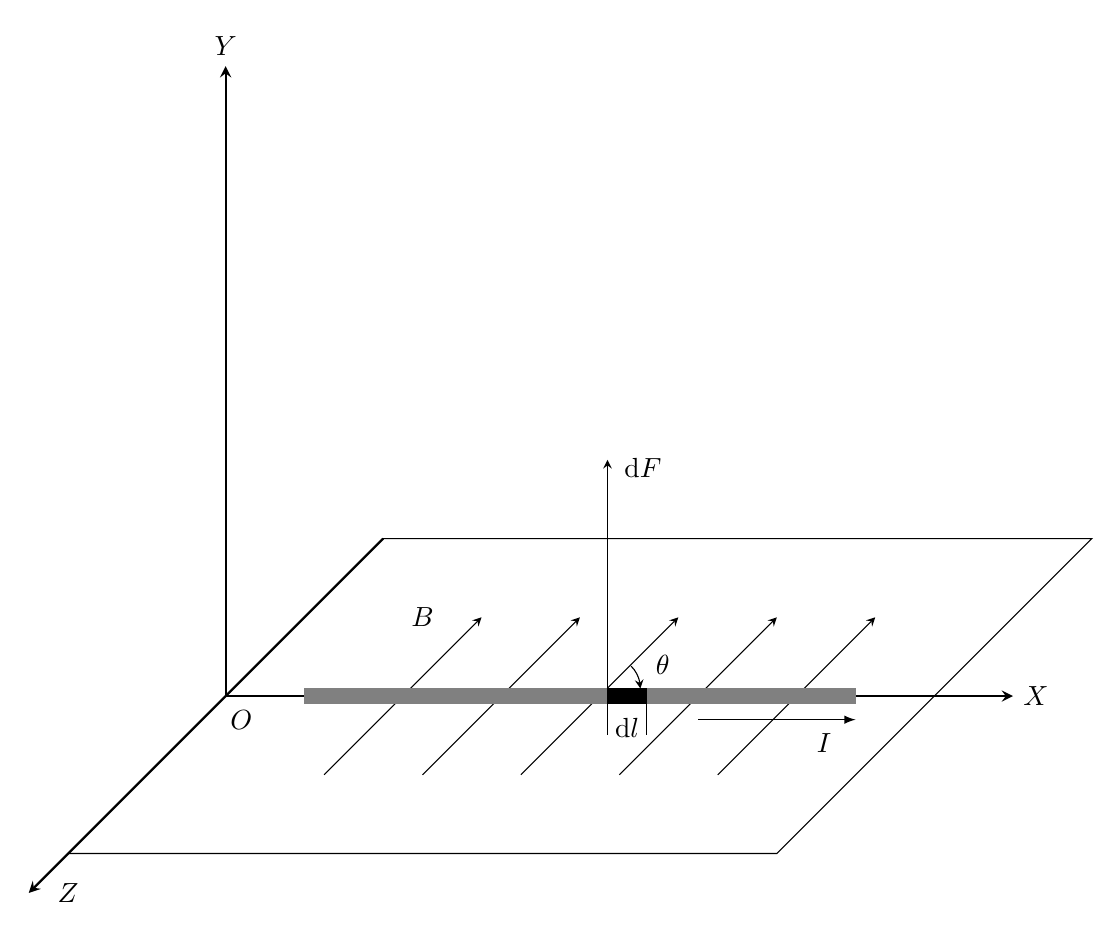
\begin{tikzpicture}[>=stealth,scale=1.0]
                \draw[->,thick](0,0)--(10,0) node[right] {$X$};
                \draw[->,thick](0,0)--(0,8) node[above] {$Y$};
                \draw[->,>=stealth,thick](2,2)--(-2.5,-2.5) node at(-2,-2.5) {$Z$};
                \draw[-](2,2)--(11,2)--(7,-2)--(-2,-2);
    
                \node at(0.2,-0.3) {$O$};

                \draw [->,>=stealth](1.25,-1)--(3.25,1);
                \draw [->,>=stealth](2.50,-1)--(4.50,1);
                \draw [->,>=stealth](3.75,-1)--(5.75,1);
                \draw [->,>=stealth](5.00,-1)--(7.00,1);
                \draw [->,>=stealth](6.25,-1)--(8.25,1);
                \node at(2.5,1.0) {$B$};

                \draw [->,>=stealth](5.15,0.38) arc(45:0:0.4);
                \node at(5.55,0.4) {$\theta$};

                \draw [->,>=stealth](4.85,0)--(4.85,3) node at(5.3,2.9) {$\dif F$};

                \fill [gray] (1,-0.1) rectangle (8,0.1);
                \fill [black] (4.85,-0.1) rectangle (5.35,0.1);
                \draw [-latex] (6,-0.3)--(8,-0.3);
                \node at(7.6,-0.6) {$I$};

                \draw[-] (4.85,0.1)--(4.85,-0.5);
                \draw[-] (5.35,0.1)--(5.35,-0.5);
                \node at(5.10,-0.4) {$\dif l$};
            \end{tikzpicture}
            \caption{通电直导线受到的磁场作用}
        \end{center}        
    \end{figure}\\
    根据安培定律和毕奥-萨伐尔定律:
    \setcounter{equation}{0}
    \begin{equation}
        \dif F=I\cdot\dif l\cdot B\cdot\sin{\theta}
    \end{equation}\\
    由于我们考虑的是匀强磁场,
    所以导线上各个电流元受到的磁场力的方向都是一致的,
    通过积分可以得到通电直导线在匀强磁场$B$中受到的总磁场力:\vspace{5pt}
    \begin{equation}
        F=\int_{L}\dif F=\int_{L} I\cdot\dif l\cdot B\cdot\sin{\theta}
    \end{equation}

\newpage

    我们设导线的起始点为$l_1$,终止点为$l_2$,求解积分:\vspace{5pt}
    \begin{align}
        F
        &=\int_{l_1}^{l_2}I\cdot\dif l\cdot B\cdot\sin{\theta}\\[3mm]
        &=I\cdot B\cdot\sin{\theta}\cdot\int_{l_1}^{l_2} dl\\[3mm]
        &=I\cdot B\cdot\sin{\theta}\cdot[\;l\;]^{l_2}_{l_1}\\[3mm]
        &=I\cdot B\cdot\sin{\theta}\cdot[\;l_2-l_1\;]
    \end{align}\\
    显然,通电直导线受到的磁场力只和导线长度有关,所以我们可以令$l=l_2-l_1$。\\[3mm]
    通电直导线受到的磁场力:
    \begin{large}
        \begin{equation*}
            F=I\cdot l\cdot B\cdot\sin{\theta}
        \end{equation*}
    \end{large}

\subsection{磁现象的电本质}
    科学家们曾经类比电场是由于电荷而产生的,
    认为磁场是由磁荷而产生的,
    但随着科学的发展,我们发现磁荷并不存在,
    我们现在认为磁场实际上是由电流产生的。\\[3mm]
    磁场是由于电流产生的,
    这样的认识可以很好的解释的磁场,
    却难以解释磁铁的磁场。\\[3mm]
    安培对此提出了分子电流假说:
    分子内部存在一种环形电流,称为环形电流。\\[3mm]
    在物体未磁化时,
    分子电流的取向是杂乱无章的,
    产生的磁场互相抵消,对外不显磁性。\\[3mm]
    在物体被磁化时,在外界磁场作用下,
    分子电流的取向基本趋向于一致,产生的磁场互相叠加,
    从而在磁体两端对外界形成较强的磁作用,在磁体的两端形成磁极。\\[3mm]
    磁体在高温或受到猛烈敲击时会失去磁性,
    这是由于在剧烈的机械运动或剧烈热运动的影响下,
    原本取向一致的分子电流重新变得杂乱无章,对外不再现磁性。\\[3mm]
    磁体产生的磁场是由于微观上的电流。\\[1mm]
    导线产生的磁场是由于宏观上的电流。\\[3mm]
    所有的磁现象都是由于电流而产生的,这就是磁现象的电本质。

\newpage

\subsection{两根平行通电直导线的相互作用}
    如图,对于两根通电直导线,
    如果我们认为导线长度$l$远远大于导线间距$r$,
    那么我们就可以应用之前得出的结论,
    首先推出导线处的磁感强度,再得出导线所受的磁场力。\\[3mm]
    对于磁场力的方向,我们可以组合使用右手螺旋定则和左手定则,具体方向如图:\\[1mm]
    \begin{figure}[h]
        \begin{center}
            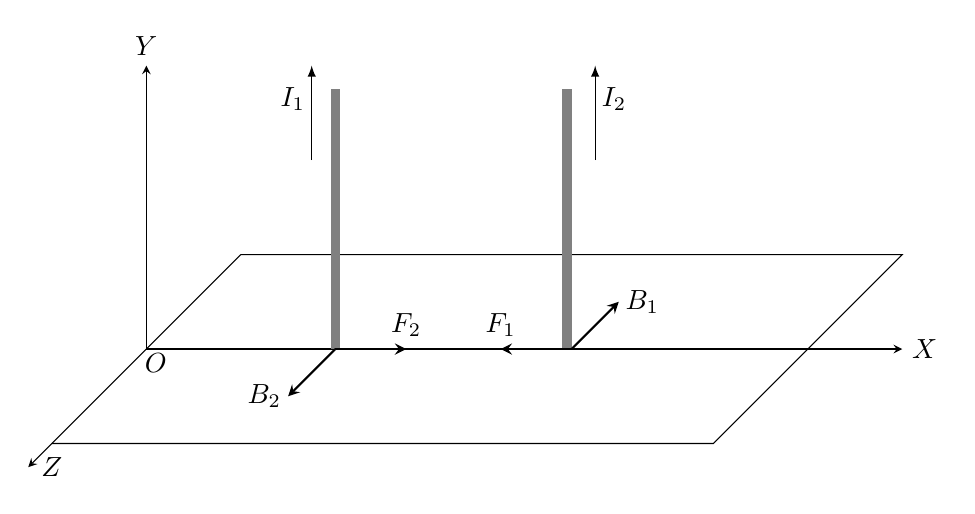
\begin{tikzpicture}[>=stealth,scale=0.6]
                \draw[->](0,0)--(16,0) node[right] {$X$};
                \draw[->](0,0)--(0,6) node[above] {$Y$};
                \draw[->,>=stealth](2,2)--(-2.5,-2.5) node at(-2,-2.5) {$Z$};
                \draw[-](2,2)--(16,2)--(12,-2)--(-2,-2);

                \node at(0.2,-0.3) {$O$};

                \fill [gray] (3.9,0) rectangle (4.1,5.5);
                \draw [-latex] (3.5,4)--(3.5,6);
                \node at(3.1,5.3) {$I_1$};

                \fill [gray] (8.8,0) rectangle (9.0,5.5);
                \draw [-latex] (9.5,4)--(9.5,6);
                \node at(9.9,5.3) {$I_2$};

                \draw [->,>=stealth,thick](4,0)--(3,-1);
                \draw [->,>=stealth,thick](9,0)--(10,1);
                \node at(2.5,-1) {$B_2$};
                \node at(10.5,1) {$B_1$};

                \draw [->,>=stealth,thick](4,0)--(5.5,0);
                \draw [->,>=stealth,thick](9,0)--(7.5,0);
                \node at(5.5,0.5) {$F_2$};
                \node at(7.5,0.5) {$F_1$};
            \end{tikzpicture}
            \caption{同向电流间的相互作用}
        \end{center}        
    \end{figure}
    \begin{figure}[h]
        \begin{center}
            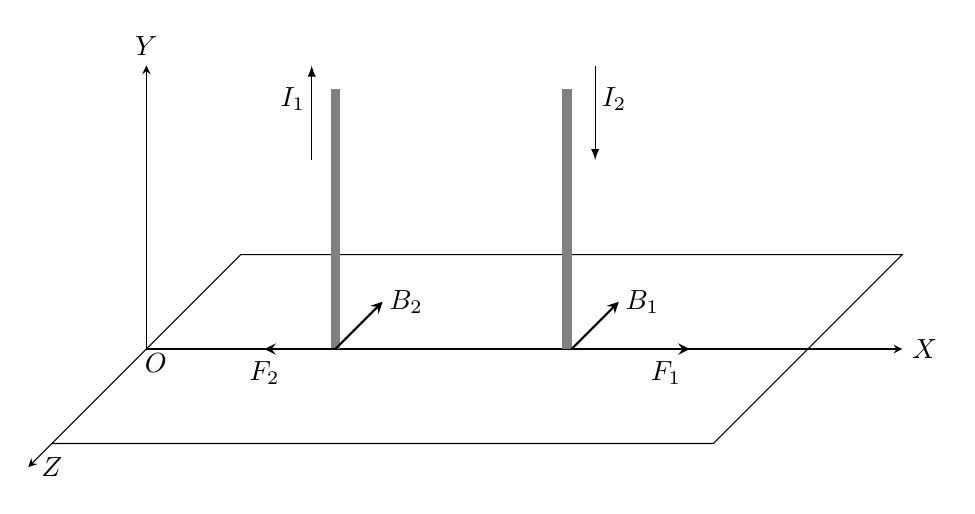
\begin{tikzpicture}[>=stealth,scale=0.6]
                \draw[->](0,0)--(16,0) node[right] {$X$};
                \draw[->](0,0)--(0,6) node[above] {$Y$};
                \draw[->,>=stealth](2,2)--(-2.5,-2.5) node at(-2,-2.5) {$Z$};
                \draw[-](2,2)--(16,2)--(12,-2)--(-2,-2);

                \node at(0.2,-0.3) {$O$};

                \fill [gray] (3.9,0) rectangle (4.1,5.5);
                \draw [-latex] (3.5,4)--(3.5,6);
                \node at(3.1,5.3) {$I_1$};

                \fill [gray] (8.8,0) rectangle (9.0,5.5);
                \draw [-latex] (9.5,6)--(9.5,4);
                \node at(9.9,5.3) {$I_2$};

                \draw [->,>=stealth,thick](4,0)--(5,1);
                \draw [->,>=stealth,thick](9,0)--(10,1);
                \node at(5.5,1) {$B_2$};
                \node at(10.5,1) {$B_1$};

                \draw [->,>=stealth,thick](4,0)--(2.5,0);
                \draw [->,>=stealth,thick](9,0)--(11.5,0);
                \node at(2.5,-0.5) {$F_2$};
                \node at(11,-0.5) {$F_1$};
            \end{tikzpicture}
            \caption{异向电流间的相互作用}
        \end{center}        
    \end{figure}\\
    对于同向的电流,两者受到的磁场力表现为吸引。\\[2mm]
    对于异向的电流,两者受到的磁场力表现为排斥。\\[6mm]
    首先我们需要得出导线处的磁感强度:
    \setcounter{equation}{0}
    \begin{equation}
        B=2k\cdot\frac{I}{r}
    \end{equation}\\
    然后我们需要得出导线所受的磁场力:
    \begin{align}
        F
        &=I\cdot l\cdot B\\[4mm]
        &=I\cdot l\cdot 2k\cdot\frac{I}{r}\\[4mm]
        &=2k\cdot\frac{I^2\cdot l}{r}
    \end{align}\\
    两条通电直导线间的磁场力:
    \begin{large}
        \begin{equation*}
            F=2k\cdot\frac{I^2\cdot l}{r}
        \end{equation*}
    \end{large}\vspace{-10pt}

\subsection{磁通量}
    磁通量指的是磁场的通量,衡量了磁场的分布情况:
    \begin{large}
        \begin{equation*}
            \Phi=B\cdot S\cdot\cos{\theta}
        \end{equation*}
    \end{large}\\
    磁通量单位:N $\cdot$ m$^2$ / A $\cdot$ m\\[3mm]
    磁通量的计算公式中的$\theta$代表磁感强度和平面垂线的夹角。\\[3mm]
    磁通量是磁感强度和面积的乘积,
    我们也可以将磁通量理解为穿过某个平面的磁感线数量。\\[3mm]
    为了纪念德国物理学家韦伯,我们用韦伯(Wb)命名磁通量单位。\vspace{5pt}

\subsubsection{高斯磁场定律}
    高斯电场定律描述了电场中闭合曲面的电通量:\vspace{5pt}
    \begin{large}
        \begin{equation*}
            \Phi=\oint_SB \cdot \dif S=0
        \end{equation*}
    \end{large}\\
    高斯磁场定律:通过闭合曲面的磁通量恒为零。\\[8mm]
    我们可以通过电场线形象的理解高斯电场定律:\\[3mm]
    1.假设一个小磁体,其磁感线由磁体N极发出,其磁感线于磁体N极汇集。\\[3mm]
    2.我们可以在磁感线的图中画出一个闭合曲线,我们会发现无论这条曲线的形状大小如何改变,
    只要这条曲线是闭合的,那么进入和离开曲面的磁感线数量相同。\\[3mm]
    3.因此闭合曲面的磁通量恒为零,与曲面形状无关。

\newpage

\subsection{洛伦兹力}
    洛伦兹力指的是磁场对运动电荷的作用力。\\[4mm]
    我们可以将导线上的电流表达为:
    \setcounter{equation}{0}
    \begin{align}
        I=n\cdot q\cdot S\cdot v
    \end{align}\\
    我们可以将导线所受的磁场力表达为:
    \begin{align}
        F=I\cdot l\cdot B\cdot \sin{\theta}
    \end{align}\\
    用$N$代表导线中的电荷总数,用$f$代表每个电荷所受的力,可以得到:\vspace{5pt}
    \begin{align}
        F=N\cdot f
    \end{align}\\
    显然导线中的总电荷数$N$可以表达为单位体积内的电荷数$n$和总体积$S\cdot l$的乘积:\vspace{5pt}
    \begin{align}
        N=n\cdot S\cdot l
    \end{align}\\
    将以上关系代入可得:
    \begin{align}
        &F=I\cdot l\cdot B\cdot \sin{\theta}\\[3mm]
        &N\cdot f=I\cdot l\cdot B\cdot \sin{\theta}\\[3mm]
        &N\cdot f=n\cdot q\cdot S\cdot v\cdot l\cdot B\cdot \sin{\theta}\\[3mm]
        &f=q\cdot v\cdot B\cdot \sin{\theta}
    \end{align}\\
    此处每个电荷所受的力$f$就是洛伦兹力。\\[4mm]
    洛伦兹力的计算公式:
    \begin{large}
        \begin{equation*}
            f=q\cdot v\cdot B\cdot\sin{\theta}
        \end{equation*}
    \end{large}

\newpage

\subsection{电磁感应}
    电磁感应现象:当穿过闭合电路的磁通量发生变化,闭合电路中就会有电流产生。\\[2mm]
    由电磁感应产生的电动势称为感应电动势,由电磁感应产生的电流称为感应电流。\\[4mm]
    法拉第电磁感应定律定量的说明了感应电动势和磁通量变化的关系。\\[3mm]
    法拉第电磁感应定律:感应电动势的大小和磁通量的变化率成正比。\\[3mm]
    法拉第电磁感应定律的数学表达:
    \begin{large}
        \begin{equation*}
            \mathscr{E}=\frac{\dif\Phi}{\dif t}
        \end{equation*}
    \end{large}\\
    楞次定律说明了感应电动势的方向和磁通量变化的关系。\\[3mm]
    楞次定律:感应电流总是要使它所产生的磁场阻碍外磁场磁通量的变化。\\

\subsubsection{动生电动势}
    动生电动势指的是由于导体和磁场发生相对运动,引起磁通量变化产生的感应电动势。\\[3mm]
    动生电动势产生的根本原因,是由于洛伦兹力对导体内电荷的作用而产生的。\\[3mm]
    如下图所示,一根金属棒在磁场中向右运动,在金属棒中的大量自由电子受到向下的洛伦兹力,
    使自由电子在金属棒的下端集中,金属棒的上端聚集了正电荷,金属棒的下端聚集了负电荷。\\
    \begin{figure}[h]
        \begin{center}
            \begin{tikzpicture}[>=stealth,scale=1.0]
                \node at(3,3) {$\times$};
                \node at(3,1) {$\times$};
                \node at(3,-1) {$\times$};
                \node at(3,-3) {$\times$};

                \node at(1,3) {$\times$};
                \node at(1,1) {$\times$};
                \node at(1,-1) {$\times$};
                \node at(1,-3) {$\times$};

                \node at(-1,3) {$\times$};
                \node at(-1,1) {$\times$};
                \node at(-1,-1) {$\times$};
                \node at(-1,-3) {$\times$};

                \node at(-3,3) {$\times$};
                \node at(-3,1) {$\times$};
                \node at(-3,-1) {$\times$};
                \node at(-3,-3) {$\times$};

                \draw (-0.2,2.8) rectangle (0.2,-2.8);

                \draw[->] (0.2,0)--(2.2,0);
                \node at(2.5,0) {$v$};

                \node at(0,2.55) {$+$};
                \node at(0,-2.6) {$-$};

                \draw (-4.5,0) circle (0.15);
                \node at(-4.5,-0.03) {$\textbf{-}$};

                \draw[->] (-4.5,0.15)--(-4.5,2.15);
                \draw[->] (-4.5,-0.15)--(-4.5,-2.15);
                \node at(-5,2.0) {$F_C$};
                \node at(-5,-2.0) {$F_A$};
            \end{tikzpicture}
            \caption{动生电动势示意图}
        \end{center}
    \end{figure}\\

\newpage

    因此金属棒中的自由电子同时受到两种力的作用,洛伦兹力($F_A$),库仑力($F_C$):\vspace{5pt}
    \setcounter{equation}{0}
    \begin{align}
        &F_C=E\cdot q\\[3mm]
        &F_A=B\cdot q\cdot v
    \end{align}\\
    显然最终洛伦兹力和库仑力会趋向于平衡:\vspace{3pt}
    \begin{align}
        &E\cdot q=B\cdot q\cdot v\\[4mm]
        &E=B\cdot v\\[4mm]
        &\frac{\mathscr{E}}{l}=B\cdot v\\[4mm]
        &\mathscr{E}=B\cdot v\cdot l
    \end{align}\\
    动生电动势的计算公式:
    \begin{large}
        \begin{equation*}
            \mathscr{E}=B\cdot l\cdot v
        \end{equation*}
    \end{large}\\
    动生电动势的计算公式与法拉第电磁感应定律等价。\\[6mm]
    动生电动势的方向判断法则:伸开右手,使得磁感线穿过右手掌心,拇指指向导体运动的方向,
    四指正方向指向导体高电势端,四指反方向指向导体低电势端。\\[2mm]
    动生电动势的方向判断法则与楞次定律等价。

\subsubsection{感生电动势}
    感生电动势指的是由于磁场的强弱发生变化,引起磁通量变化产生的感应电动势。\\[3mm]
    感生电动势产生的根本原因,是由于变化的磁场产生的涡旋电场。\\[3mm]
    感生电动势的计算公式:
    \begin{large}
        \begin{equation*}
            \mathscr{E}=\frac{\dif\Phi}{\dif t}
        \end{equation*}
    \end{large}\\
    感生电动势的计算公式与法拉第电磁感应定律等价。\\[6mm]
    感生电动势的方向判断法则:当外磁场增强时,感应电流的磁场方向与外磁场的磁场方向相反,
    当外磁场减弱时,感应电流的磁场方向与外磁场的磁场方向相同。\\[2mm]
    感生电动势的方向判断法则与楞次定律等价。

\newpage

\subsubsection{电磁感应中的电流和电荷量}
    设一个闭合金属框的电阻为$R$通过磁场强度为$B$的匀强磁场,其切割磁感线的部分长度为$l$。\\[3mm]
    设金属框在磁场中的速度为$v$,设金属框在磁场中的位移是$s$。\\[4mm]
    显然过程中金属框中的电流可以表示为:
    \begin{align}
        I
        &=\frac{E}{R}\\[4mm]
        &=\frac{B\cdot l\cdot v}{R}
    \end{align}\\
    显然过程中金属框中的电荷量可以表示为:
    \setcounter{equation}{0}
    \begin{align}
        Q
        &=\int I\cdot\dif t\\[4mm]
        &=\int \frac{B\cdot l\cdot v}{R}\cdot\dif t\\[4mm]
        &=\frac{B\cdot l}{R}\cdot\int v\cdot\dif t\\[4mm]
        &=\frac{B\cdot l\cdot s}{R} 
    \end{align}\\
    电磁感应中的电流表达式:
    \begin{large}
        \begin{equation*}
            I=\frac{B\cdot l\cdot v}{R}
        \end{equation*}
    \end{large}\\
    电磁感应中的电荷量表达式:
    \begin{large}
        \begin{equation*}
            Q=\frac{B\cdot l\cdot s}{R}
        \end{equation*}
    \end{large}\\
    从中我们发现感应电荷量大小,只与在磁场中的位移大小有关,而与在磁场中的速度大小无关。

\newpage

\section{电磁波}

\subsection{电磁波的类型}
    麦克斯韦认为,变化的电场产生磁场,变化的磁场产生电场,电场和磁场是电磁场的不同侧面。\\[3mm]
    电磁波是由于空间中电场和磁场交替变换并由近及远向周围的空间传播而产生。\\[3mm]
    电磁波在真空中的传播速度等于光速,电磁波是一种横波,其传播不需要介质。\\[5mm]
    以下列出了各个频率电磁波的名称:\vspace{5pt}
    \begin{table}[h]
        \begin{center}
            \begin{tabular}{l|l|l|l}
                \hline
                电磁波类型~~~~~~~~&电磁波具体类型~~~~~~~~&波长~~~~~~~~~~~~~~~~~~~~~~~~&频率~~~~~~~~~~~~~~~~~~~~~~~~\\ \hline
                \multirow{8}*{无线电波}
                &甚长波&$>10000$~m&$<30$~KHz\\ \cline{2-4}
                &长波&$>1000$~m&$<300$~KHz\\ \cline{2-4}
                &中波&$>100$~m&$<3$~MHz\\ \cline{2-4}
                &短波&$>10$~m&$<30$~MHz\\ \cline{2-4}
                &米波&$>1$~m&$<300$~MHz\\ \cline{2-4}
                &分米波&$>100$~mm&$<3$~GHz\\ \cline{2-4}
                &厘米波&$>10$~mm&$<30$~GHz\\ \cline{2-4}
                &毫米波&$>1$~mm&$<300$~GHz\\ \cline{1-4}
                \multirow{3}*{红外线}
                &远红外线&$>30$~$\upmu$m&$<10$~THz\\ \cline{2-4}
                &中红外线&$>3$~$\upmu$m&$<100$~THz\\ \cline{2-4}
                &近红外线&$>0.75$~$\upmu$m&$<400$~THz\\ \cline{1-4}
                \multirow{6}*{可见光}
                &红光&$622-750$~nm&$400-482$~THz\\ \cline{2-4}
                &橙光&$597-622$~nm&$482-503$~THz\\ \cline{2-4}
                &黄光&$577-597$~nm&$503-520$~THz\\ \cline{2-4}
                &绿光&$492-577$~nm&$520-610$~THz\\ \cline{2-4}
                &蓝光&$455-492$~nm&$610-659$~THz\\ \cline{2-4}
                &紫光&$400-455$~nm&$750-857$~THz\\ \cline{1-4}
                \multirow{4}*{紫外线}
                &近紫外线&$>300$~nm&$<1000$~THz\\ \cline{2-4}
                &中紫外线&$>200$~nm&$<1500$~THz\\ \cline{2-4}
                &远紫外线&$>122$~nm&$<2459$~THz\\ \cline{2-4}
                &极紫外线&$>10$~nm&$<30$~PHz\\ \cline{1-4}
                \multirow{1}*{伦琴射线}
                &伦琴射线&$>0.01$~nm&$<30$~EHz\\ \cline{1-4}
                \multirow{1}*{伽马射线}
                &伽马射线&$<0.01$~nm&$>30$~EHz\\ \cline{1-4}
            \end{tabular}
            \caption{电磁波的类型}
        \end{center}
    \end{table}\\
    需要说明的是,伦琴射线和伽马射线在频率和波长上实际有一定重叠,通常按照来源进行区分,
    伦琴射线是原子核外电子在能级间跃迁时放出的,伽马射线是原子核在能级间跃迁时放出的。

\newpage

    电磁波的波长和频率间存在以下关系:
    \begin{large}
        \begin{equation*}
            \lambda\cdot\nu=c
        \end{equation*}
    \end{large}\\
    这是由于电磁波的传播速度均为光速,因此对于电磁波来说,波长和频率是两个等价的物理量。\\

\subsection{光的波动性}
    光的波动性需要由双缝干涉实验证明。\\[3mm]
    光的波动说认为光的一种振动,以波的形式向周围传播。\\[3mm]
    光的干涉:两列频率相同相差恒定的相干光波叠加后,某些部分始终加强,某些部分始终减弱。\\[5mm]
    该实验的关键在于如何获取两列相干光波,即如何制造两个相干光源。\\[3mm]
    第一步需要使用单缝屏,使得一束单色光照射到缝中,由此形成一个光源。\\[3mm]
    第二步需要使用双缝屏,由于光波会同时传到两个缝中,所以形成了两个相干光源。\\[3mm]
    第三步需要使用光屏,两列相干光波在干涉的作用下,投影在光屏上形成明暗相间的条纹。\\[3mm]
    干涉现象是波的独有特性,因此证明了光的波动性。\\[5mm]
    由于该实验首先由英国物理学家托马斯·杨完成,因此称为杨氏双缝干涉实验。\vspace{8pt}
    \begin{figure}[h]
        \begin{center}
            \begin{tikzpicture}[>=stealth,scale=1.0]

                \fill[fill=gray] (-2.1,3) rectangle (-1.9,0.2);
                \fill[fill=gray] (-2.1,-0.2) rectangle (-1.9,-3);

                \fill[fill=gray] (-0.1,3) rectangle (0.1,1.2);
                \fill[fill=gray] (-0.1,0.8) rectangle (0.1,-0.8);
                \fill[fill=gray] (-0.1,-1.2) rectangle (0.1,-3);

                \fill[fill=black] (1.9,3) rectangle (2.1,-3);

                \draw (-4,0) circle (0.2);
                \node at(-4,0) {$\mathbf{\times}$};
                
                \node at(-4,-0.8) {光源};
                \node at(-2,-3.8) {单缝屏};
                \node at(0,-3.8) {双缝屏};
                \node at(2,-3.8) {光屏};

                \draw[->] (-3.5,0)--(-2.1,0);
                \draw[->] (-1.9,0.1)--(-0.1,1);
                \draw[->] (-1.9,-0.1)--(-0.1,-1);

                \node at(2.3,2.6) {\footnotesize 亮};
                \node at(2.3,2.2) {\footnotesize 暗};
                \node at(2.3,1.8) {\footnotesize 亮};
                \node at(2.3,1.4) {\footnotesize 暗};
                \node at(2.3,1.0) {\footnotesize 亮};
                \node at(2.3,0.6) {\footnotesize 暗};
                \node at(2.3,0.2) {\footnotesize 亮};
                \node at(2.3,-0.2) {\footnotesize 暗};
                \node at(2.3,-0.6) {\footnotesize 亮};
                \node at(2.3,-1.0) {\footnotesize 暗};
                \node at(2.3,-1.4) {\footnotesize 亮};
                \node at(2.3,-1.8) {\footnotesize 暗};
                \node at(2.3,-2.2) {\footnotesize 亮};
                \node at(2.3,-2.6) {\footnotesize 暗};

            \end{tikzpicture}
            \caption{杨氏双缝干涉实验示意图}
        \end{center}
    \end{figure}\\
\newpage

\subsection{光的粒子性}
    光的粒子性需要由光电效应实验证明。\\[3mm]
    光的粒子说认为光是一种粒子,以一定的速度进行传播。\\[3mm]
    光电效应:在可见光或不可见光的照射下,物体发射出电子的现象,这些电子称为光电子。\\[6mm]
    光电效应具有极限频率的特点,对于某一特定的金属材料,只有入射光的频率高于其极限频率,才能产生光电效应,
    若入射光的频率低于其极限频率,无论光的强度如何,无论照射时间如何,也都不能产生光电效应,
    极限频率通常记作$\nu_0$,极限波长通常记作$\lambda_0$。\\[6mm]
    光电效应无法通过光的波动说解释。\\[3mm]
    按照波动理论,光的能量是由光的振幅决定,光的能量与光的频率无关,
    因此无论频率如何,只要光的振幅足够强或照射时间足够长,就可以产生光电效应,但这无法解释极限频率的存在。\\[6mm]
    光电效应可以通过光的粒子说解释。\\[3mm]
    按照粒子理论,光在空间中传播是不连续的,或者说是一份一份的,每一份称为一个光子。\\[3mm]
    光子能量和频率成正比:
    \begin{large}
        \begin{equation*}
            E=h\cdot \nu
        \end{equation*}
    \end{large}\\
    光子能量公式中的比例系数$h$称为普朗克常数,其取值为$h=6.63\times 10^{-34}$~J$\cdot$s。\\[3mm]
    光子照射到金属上时,光子的能量可以被电子全部吸收,电子后吸收能量可能向各个方向运动,电子的能量损失各有不同,
    电子克服金属离子的引力所需做的最少的功称为逸出功$W_0$。\\[3mm]
    光子的能量如果低于逸出功,电子始终无法离开金属形成光电子,光的能量只和光的频率相关,
    因此低于某一频率的光所具有的能量无法产生光电效应,这就很好的解释了极限频率的存在。\\

\subsection{波粒二象性}
    光即具有波动性,光也具有粒子性,无法使用其中一种解释光的行为,这就是光的波粒二象性。\\[3mm]
    实际上所有的电磁波均具有波粒二象性:\\[3mm]
    对于频率较低或波长较长的电磁波,例如无线电波,其波动性较为明显,较难观察到粒子性。\\[3mm]
    对于频率较高或波长较短的电磁波,例如伽马射线,其粒子性较为明显,较难观察到波动性。\\[3mm]
    
\newpage

\section{原子物理}

\subsection{原子结构的探索}
    自从道尔顿提出物体是由原子组成开始,科学家们普遍认为原子是不可分割的最小质点。\vspace{5pt}

\subsubsection{汤姆孙和原子的葡萄干蛋糕模型}
    汤姆孙的阴极射线实验揭示了原子中存在电子。\\[3mm]
    汤姆孙通过数十年的研究证明了阴极射线是带负电的微粒流,通过对阴极射线的核质比的测定,
    发现其是氢离子的2000倍,这说明存在两种可能的情况:\\[3mm]
    1.阴极射线粒子的电荷$q$~~\,远大于氢离子。\\[3mm]
    2.阴极射线粒子的质量$m$远小于氢离子。\\[3mm]
    汤姆孙随后较为粗略的测量了阴极射线粒子的电荷量,发现其与氢离子的电荷量是大致相同的,这种粒子随后被称为电子,
    由于电子的质量远小于已知的氢离子的质量,说明原子中存在电子,说明原子并不是不可分割的,说明原子是存在内部结构的。\\[3mm]
    汤姆孙针对实验结果,提出了原子的葡萄干蛋糕模型:\\[3mm]
    原子中充斥着带正电的流体,其中镶嵌着若干带负电的电子,因此原子对外不显电性。\\

\subsubsection{卢瑟福和原子的行星模型}
    卢瑟福的阿尔法粒子散射实验揭示了原子的核式结构。\\[3mm]
    卢瑟福对其老师汤姆孙提出的原子模型并不满意,使用了其发现的$\alpha$粒子对金箔进行轰击。\\[3mm]
    卢瑟福发现大部分$\alpha$粒子直接穿过金箔,少部分发生小角度偏转,极少部分发生大角度偏转。\\[3mm]
    但是实验测得的和理论预测的发生大角度偏转的$\alpha$粒子概率严重不符:
    \begin{table}[h]
        \begin{center}
            \begin{tabular}{l|l}
                \hline
                理论预测的发生大角度偏转的$\alpha$粒子概率~~~~&$1/10^{35}$~~~~\\ \hline
                实验测得的发生大角度偏转的$\alpha$粒子概率~~~~&$1/8000$~~~~\\ \hline
            \end{tabular}
            \caption{发生大角度偏转的$\alpha$粒子概率对比}
        \end{center}
    \end{table}\\
    卢瑟福经过计算认为,如果按照汤姆孙提出的葡萄干蛋糕模型,正电荷均匀的分布在原子中,会无法解释观察到现象,
    只有原子中所有质量集中于很小一处,才有可能发生如此大角度的偏转。\\[3mm]
    卢瑟福针对实验结果,提出了原子的行星模型:\\[3mm]
    原子的中存在带正电的原子核,原子核体积很小但集中了大部分质量,电子绕原子核高速旋转。

\newpage

\subsection{核衰变}
    核衰变指的是一种原子核通过放出射线而变为另一种原子核的过程。\\[3mm]
    核衰变可以分为三类:$\alpha$衰变,$\beta^-$衰变,$\beta^+$衰变。\\[5mm]
    在$\alpha$衰变中,原子核抛出两个质子和两个中子,组成一个$\alpha$粒子,以$\alpha$射线的形式放出。\\[3mm]
    以下列出了一个$\alpha$衰变的核反应方程式:
    \begin{center}
        \ce{^{238}_{92}U -> ^{234}_{90}Th + ^{4}_{2}He}\\[5mm]
    \end{center}
    在$\beta^-$衰变中,原子核中的中子变为质子和负电子,负电子即$\beta^-$粒子,以$\beta-$射线的形式放出。\\[3mm]
    以下列出了一个$\beta^-$衰变的核反应方程式:
    \begin{center}
        \ce{^{234}_{90}Th -> ^{234}_{91}Pa + ^{0}_{-1}e^{-}}\\[5mm]
    \end{center}
    在$\beta^+$衰变中,原子核中的质子变为中子和正电子,正电子即$\beta^+$粒子,以$\beta+$射线的形式放出。\\[3mm]
    以下列出了一个$\beta^+$衰变的核反应方程式:
    \begin{center}
        \ce{^{30}_{15}P -> ^{30}_{14}Si + ^{0}_{+1}e^{+}}\\[5mm]
    \end{center}
    以上三种衰变方式中,由于衰变后的原子核在能级间跃迁,所以均会放出$\gamma$射线。\\[6mm]
    下表对比了三种衰变方式:\vspace{5pt}
    \begin{table}[h]
        \begin{center}
            \begin{tabular}{l|l|l|l|l}
                \hline
                衰变类型~~~~&质子数P~~~~&中子数N~~~~&相对原子质量~~~~&元素周期表上的变化~~~~\\ \hline
                $\alpha~~\,$衰变&$-2$&$-2$&$-4$&向前移动两格\\ \hline
                $\beta^-$衰变&$+1$&$-1$&$~0$&向后移动一格\\ \hline
                $\beta^+$衰变&$-1$&$+1$&$~0$&向前移动一格\\ \hline
            \end{tabular}
            \caption{三种衰变方式的对比}
        \end{center}
    \end{table}\\
    需要说明的是,$\beta^+$衰变只存在于人工合成的放射性同位素,不存在于天然放射现象。\\[3mm]
    因此一般来说,$\beta$衰变指的是$\beta^-$衰变,$\beta$粒子指的是$\beta^-$粒子,$\beta$射线指的是$\beta^-$射线。

\newpage

\subsubsection{半衰期}
    半衰期指的是放射性元素的原子核有半数发生衰变所需的时间。\\[3mm]
    半衰期越长代表这种放射性元素越稳定。\\[3mm]
    半衰期越短代表这种放射性元素越不稳定。\\[3mm]
    需要说明的是,半衰期需要建立在大量原子上,半衰期无法预测少量原子的变化情况。\\

\subsubsection{原子核的天然放射}
    天然放射现象最早是由法国物理学家贝克勒尔发现,之后科学家发现将放射源放置在电场中时,
    放出的射线分为三束,带正电的称为$\alpha$射线,带负电的称为$\beta$射线,不带电的称为$\gamma$射线。\\[3mm]
    下表对比了三种射线的性质:
    \begin{table}[h!]
        \begin{center}
            \begin{tabular}{l|l|l|l|l}
                \hline
                射线类型~~~~&物理本质~~~~~~~~&穿透能力~~~~&电离能力~~~~&速度~~~~\\ \hline
                $\alpha$射线&高速氦离子流&无法穿透纸张&较强&$0.10c$\\ \hline
                $\beta$射线&高速电子流&可以穿透数毫米厚的铝板&较弱&$0.90c$\\ \hline
                $\gamma$射线&高速光子流&可以穿透数厘米厚的铅板&较弱&$1.00c$\\ \hline
            \end{tabular}
            \caption{三种射线性质的对比}
        \end{center}
    \end{table}\\
    由于放射性物质是连续衰变的,有的发生$\alpha$衰变,有的发生$\beta$衰变,所以会同时放出三种射线。\\
    
\subsubsection{原子核的人工转变}
    通过$\alpha$粒子轰击氮原子可以产生质子:
    \begin{center}
        \ce{^{14}_{7}N + ^{4}_2{He} -> ^{17}_{8}O + ^1_1p}\\[5mm]
    \end{center}
    通过$\alpha$粒子轰击铍原子可以产生中子:
    \begin{center}
        \ce{^{9}_{4}Be + ^{4}_2{He} -> ^{12}_{6}O + ^1_0n}\\[5mm]
    \end{center}
    质子和中子的质量几乎是相等的,质子带正电荷,中子不带电荷。\\[3mm]
    质子和中子是共同组成原子核的部分,两者可以统称为核子。\\[3mm]
    由于中子流和$\gamma$射线性质相似,穿透能力强,电场中不发生偏转,因此最初被误认为是$\gamma$射线,
    直到卢瑟福的学生查德威克通过进一步研究发现其速度仅有$0.1c$,最终发现这是一种新的粒子。

\newpage

\subsection{核能}
    原子核的半径很小,依照库伦定律,质子和质子间存在极大的斥力会导致质子高速飞散,
    但是原子核是稳定的,所以必然存在某种力可以抵消库仑力的作用,使核子结合在一起。\\[3mm]
    这种力称为核力,它存在于质子和质子间,也存在于质子和中子间,还存在于中子和中子间。\\[3mm]
    核力的作用力很强,可以克服库仑力使得质子和质子结合在一起。\\[3mm]
    核力的作用距离很短,只存在于相邻的核子间起作用,超出这个距离则迅速减小至零。\\[5mm]
    当两个核子分离时,会吸收巨大的能量,
    例如氘原子分解形成质子和中子的过程中:
    \begin{center}
        \ce{^2_1H + $\gamma$ -> ^1_1p + ^1_0n}\\[7mm]
    \end{center}
    当两个核子结合时,会放出巨大的能量,
    例如质子和中子结合形成氘原子的过程中:
    \begin{center}
        \ce{^1_1p + ^1_0n -> ^2_1H + $\gamma$}\\[7mm]
    \end{center}
    核子结合时需要放出能量,核子分解时需要吸收能量,这部分能量称为原子的结合能。\\[3mm]
    结合能可以通过爱因斯坦质能方程计算:
    \begin{large}
        \begin{equation*}
            E=m\cdot c^2
        \end{equation*}
    \end{large}\\
    爱因斯坦质能方程表明,物体的能量与物体的质量成正比。\\[3mm]
    爱因斯坦质能方程说明,既然核子结合后的能量会减小,那么核子结合后的质量也会减小。\\[3mm]
    我们将组成原子核的核子和原子核整体间的质量差,称为核的质量亏损。\\[6mm]
    在原子物理学中,质量单位常用原子质量单位(u)表示:
    \begin{large}
        \begin{equation*}
            1\text{u}=1.66\times 10^{-27}\text{kg}
        \end{equation*}
    \end{large}\\
    在原子物理学中,能量单位常用兆电子伏(MeV)表示:
    \begin{large}
        \begin{equation*}
            1\text{Mev}=1.60\times 10^{-13}\text{J}
        \end{equation*}
    \end{large}\\
    根据爱因斯坦质能方程,两者存在以下关系:
    \begin{large}
        \begin{equation*}
            1\text{u}=931.5\text{MeV}
        \end{equation*}
    \end{large}

\newpage

    如果将一个原子核的结合能除以原子核的核子数,得到的结果称为核子的平均结合能。\\[3mm]
    平均结合能越大,原子核就更难拆开,原子核就更加稳定。\\[3mm]
    平均结合能越小,原子核就更易拆开,原子核就更加不稳定。\\[6mm]
    一般来说,平均结合能随质量数的增加,先快速上升,后缓慢下降。\\[3mm]
    由此可见,轻核的平均结合能显著低于质量中等的原子核。\\[3mm]
    由此可见,重核的平均结合能略微低于质量中等的原子核。

\subsection{核裂变}
    核裂变指的是重核变为多个中等核的过程,核裂变会释放大量能量。\\[3mm]
    核裂变利用的是重核的平均结合能略微低于质量中等的原子核的特性。\\[3mm]
    假设有$N$个核子,组成重核放出的能量为$N\cdot E_1$,组成中等核放出的能量为$N\cdot E_2$,
    因为$E_2>E_1$,所以$N\cdot E_2>N\cdot E_1$,由此可见重核变为中等核的过程重要额外放出能量。\\[3mm]
    由于重核的平均结合能是略微低于中等核,所以核裂变放出的能量是小于核聚变。\\[5mm]
    以下列出了一个核裂变的方程:
    \begin{center}
        \ce{^{235}_{114}U + ^1_0n -> ^{141}_{56}Ba + ^{92}_{36}Kr + 3^1_0n}\\[6mm]
    \end{center}
    核裂变需要中子轰击,核裂变同时产生中子,因此在适当的条件下,核裂变所产生的中子可以维持自身的持续进行,
    这种反应称为链式反应,可以维持链式反应的最小体积称为临界体积。

\subsection{核聚变}
    核聚变指的是多个轻核变为中等核的过程,核聚变会释放大量能量。\\[3mm]
    核聚变利用的是轻核的平均结合能显著低于质量中等的原子核的特性。\\[3mm]
    假设有$N$个核子,组成轻核放出的能量为$N\cdot E_1$,组成中等核放出的能量为$N\cdot E_2$,
    因为$E_2>E_1$,所以$N\cdot E_2>N\cdot E_1$,由此可见轻核变为中等核的过程重要额外放出能量。\\[3mm]
    由于轻核的平均结合能是显著低于中等核,所以核聚变变放出的能量是大于核裂变。\\[5mm]
    以下列出了一个核聚变的方程:
    \begin{center}
        \ce{^2_1H + ^3_1H -> ^4_2He + ^1_0n}\\[6mm]
    \end{center}
    核聚变需要通过极大的能量使得原子核克服库伦斥力,使其能接近到核力作用范围内才能发生,
    因此利用核聚变的氢弹需要通过利用核裂变的原子弹产生的巨大能量来引爆。

\end{document}